%% Based on techreport.tex template as sent by Erik Burger on 2023-11-20
%% 
%% Karlsruhe Institute of Technology
%% Institute for Program Structures and Data Organization
%% Chair for Software Design and Quality (SDQ)
%%
%% Dr.-Ing. Erik Burger
%% burger@kit.edu
%%
%% See https://sdq.kastel.kit.edu/wiki/Dokumentvorlagen
%%
%% Version 1.0, 2023-11-20

%% Available page modes: oneside, twoside
%% Available languages: english, ngerman
%% Available modes: draft, final (see README)
\documentclass[oneside, ngerman]{sdqtechreport}

%% ---------------------------------
%% | Information about the document |
%% ---------------------------------

%% Name of the group and authors
\author{Paul Buda, Martin Scheuermann, Stephan Schneider, \\
Simon Schütz und Nils Seibert}

%% Title (and possibly subtitle) of the thesis
\title{Entwurfsdokument}

\subtitle{zur Android-App Neptune}

%% You can put a logo in the ``logos'' directory and include it here
%% instead of the SDQ logo
% \grouplogo{myfile}
%% Alternatively, you can disable the group logo
% \nogrouplogo

\date{12.01.2024}

%% For example texts -- please remove in the final version
\usepackage{blindtext}

%% ====================================
%% ====================================
%% ||                                ||
%% || Beginning of the main document ||
%% ||                                ||
%% ====================================
%% ====================================
\begin{document}

%% Set PDF metadata
\setpdf



%% Set the title
\maketitle

%% ------------------------
%% |   Table of Contents  |
%% ------------------------
\tableofcontents

%% -----------------
%% |   Main part   |
%% -----------------
\cleardoublepage

%% -------------------
%% | Example content |
%% -------------------

\chapter{Änderungen zum Pflichtenheft}
\label{chap:Änderungen zum Pflichtenheft}

\begin{itemize}
    \item Als neue Entwicklungsumgebung der App wird nun Android Studio Hedgehog Version 2023.1.1 verwendet, da ein neues Update für Android Studio herausgekommen ist.
    \item Für die Spotify-API wird ein fester Zeitpunkt festgelegt, an welchem die gewünschte Funktionalität der API sichergestellt wurde. Dieser Zeitpunkt ist der 12.01.2024 um 14 Uhr.
    \item Die Mindestanforderung an die für die Ausführung der App benötigten Android Version wird von Version 7.0 auf Version 8.0 erhöht, da für die Verbindung mit dem Server mindestens die API 26 benötigt wird.
    \item In der HostControlView werden zwei weitere Buttons eingeführt: Ein ''Pause/Abspiel''- und ein ''Überspringen''-Button, welche die entsprechende Funktionalität an Spotify weitergeben. Dies vereinfacht das Abspielen von Musik.
    \item Die funktionale Anforderung F 7.5, welche aussagt, dass jeder Track in der Queue vom Host per Drag-and-Drop verschoben werden kann, wird verändert. Die Tracks in der Queue können nun vom Host nur noch mithilfe von Buttons mit dem oberen oder unteren Track getauscht werden und die Drag-and-Drop Funktion wird entfernt.
    \item Die Queue der App ist nicht mit derjenigen innerhalb von Spotify synchronisiert, da die Spotify-API diese Funktion nicht anbietet. Stattdessen wird als nächster Track immer derjenige abgespielt, der sich zu dem Zeitpunkt ganz oben in der Queue der App befindet.
\end{itemize}


\chapter{System}
\label{chap:System}

\begin{figure}[h]
    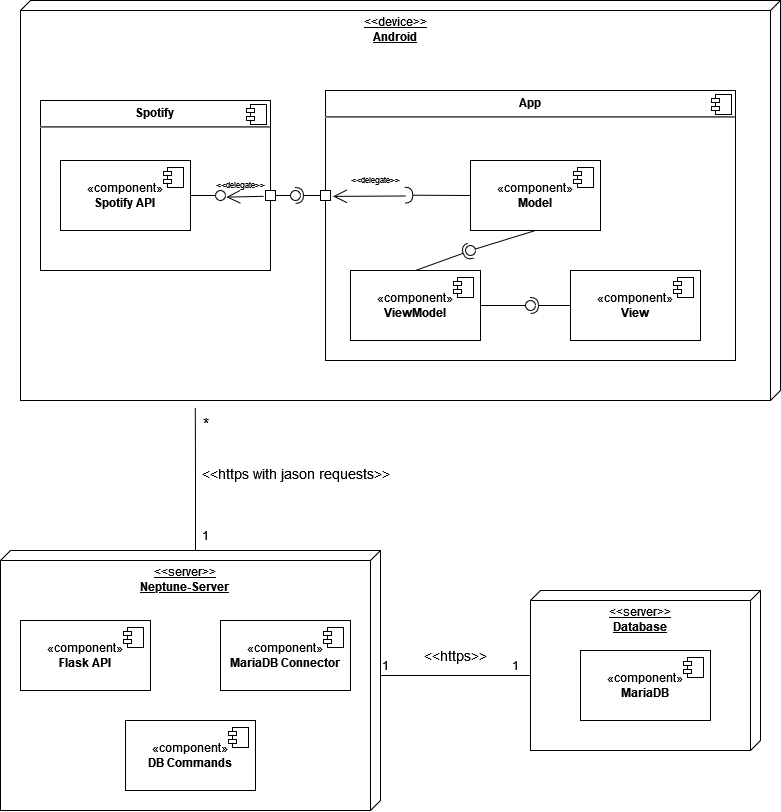
\includegraphics[width = 16cm]{LATEX/Entwurf/Graphics/Component-Diagram.png}
    \caption{Verteilungsdiagramm}
    \label{fig:Verteilungsdiagramm}
\end{figure}

\vspace{2cm}

Das gesamte System von Neptune besteht aus drei Teilen: Der Android App, dem Neptune Server und einer Datenbank.

Die App bildet den Front-End Teil des Systems und ist die von den Nutzern benutzte Hauptanwendung auf den Android Geräten. Die App kann mithilfe der Spotify API mit einem Spotify Konto verknüpft werden, was für einige Funktionalitäten erforderlich ist.

Der Server und die Datenbank bilden gemeinsam den Back-End-Teil des Systems. Der Server enthält die einzelnen Neptune Sessions und dient als Verbindung zwischen der App und der Datenbank. Die Datenbank enthält alle für eine Session relevanten Daten.

Der Server und die App kommunizieren mithilfe von JSON Objekten über eine https Verbindung. Der Server kommuniziert über SQL Anfragen mit der Datenbank.

\chapter{App}
\label{chap:App}

Die Android App wird mithilfe des Entwurfsmusters Model View ViewModel (MVVM) entwickelt. Die hierbei verwendete Programmiersprache ist Kotlin.
Im Entwurf orientieren wir uns an den Architekturempfehlungen von Android. Eine Empfehlung von Android ist die Umsetzung des MVVM-Entwurfsmusters entsprechend der unten stehenden Grafik. Diese Architekturempfehlung übernehmen wir so weit möglich für unseren Entwurf.

\begin{center}
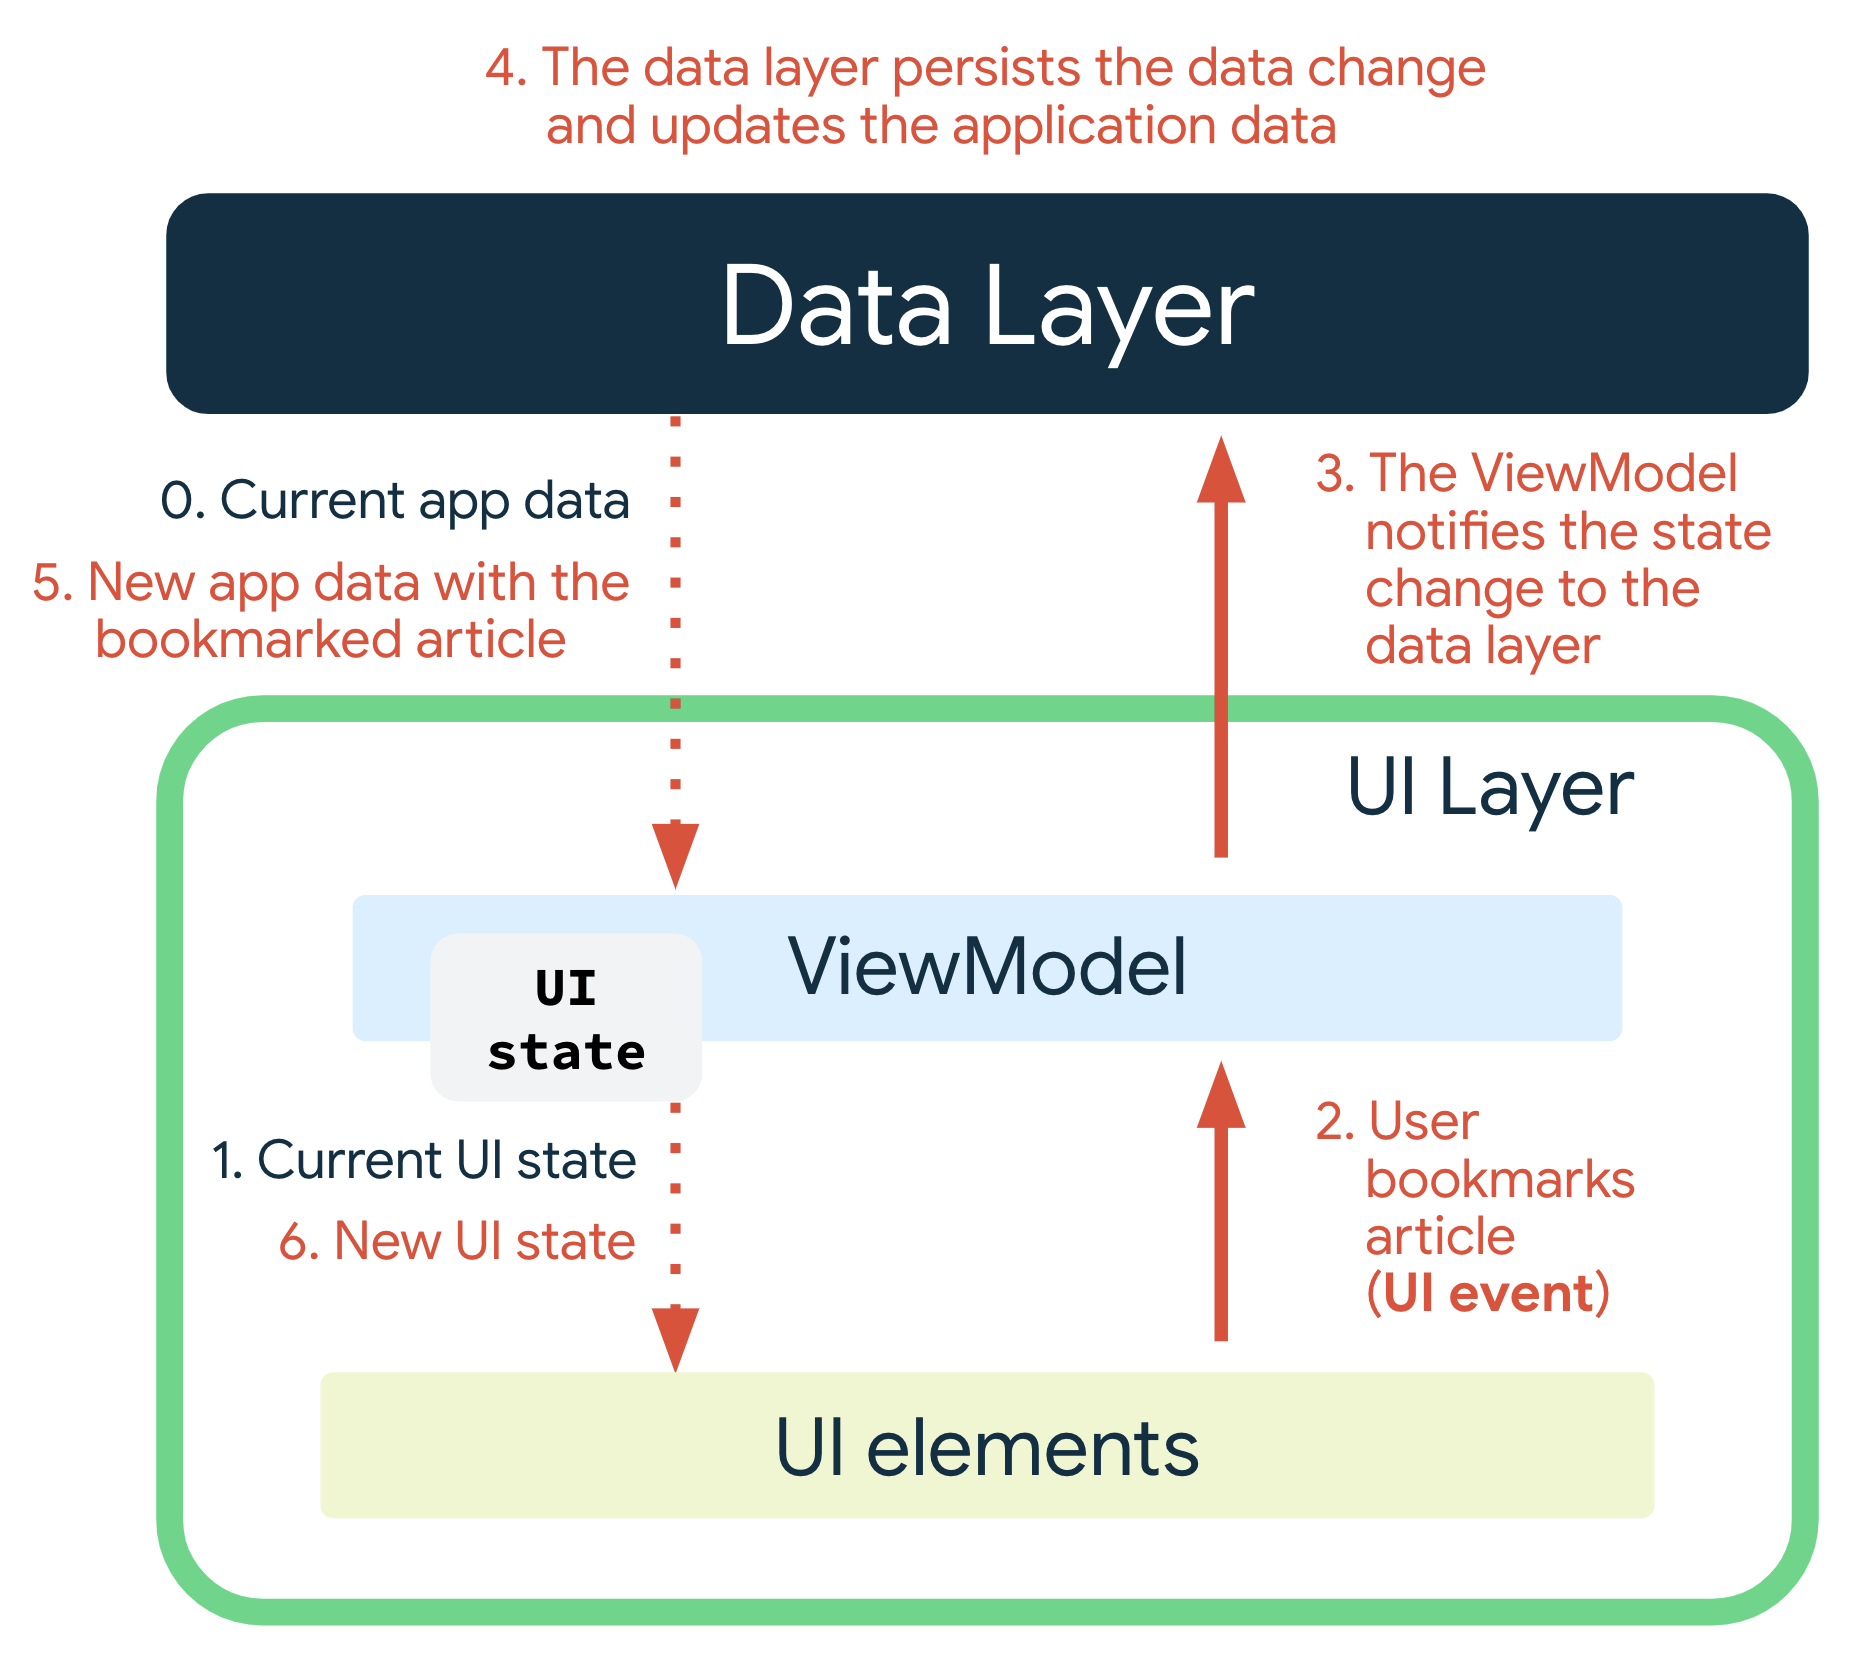
\includegraphics[width = 10cm]{LATEX/Entwurf/Graphics/Android_MVVM.png}
\captionof{figure}{Android Empfehlung - MVVM\\
\url{https://developer.android.com/topic/architecture/ui-layer} (12.01.2024)}
\end{center}


\section{Model}
\label{sec:App:Model}
Alle im folgenden genannten Pakete und Klassen liegen im Paket model. Das Model enthält die Daten im Frontend und führt die Programmlogik auf den Daten aus. Da die für Android-Apps übliche Model-ModelView-View-Aufteilung keinen Controller enthält, läuft auch die Kommunikation mit dem  Backend und Spotify über Pakete im Model.
Um die UML-Diagramme übersichtlich zu halten, sind Getter- und Setter-  Methoden nicht in den Diagrammen enthalten. Sie werden aber in den Klassenbeschreibungen beschrieben.
Das KotlinDoc der Pakete ist in Englisch verfasst, damit kann das KotlinDoc direkt für die Implementierung übernommen werden.


<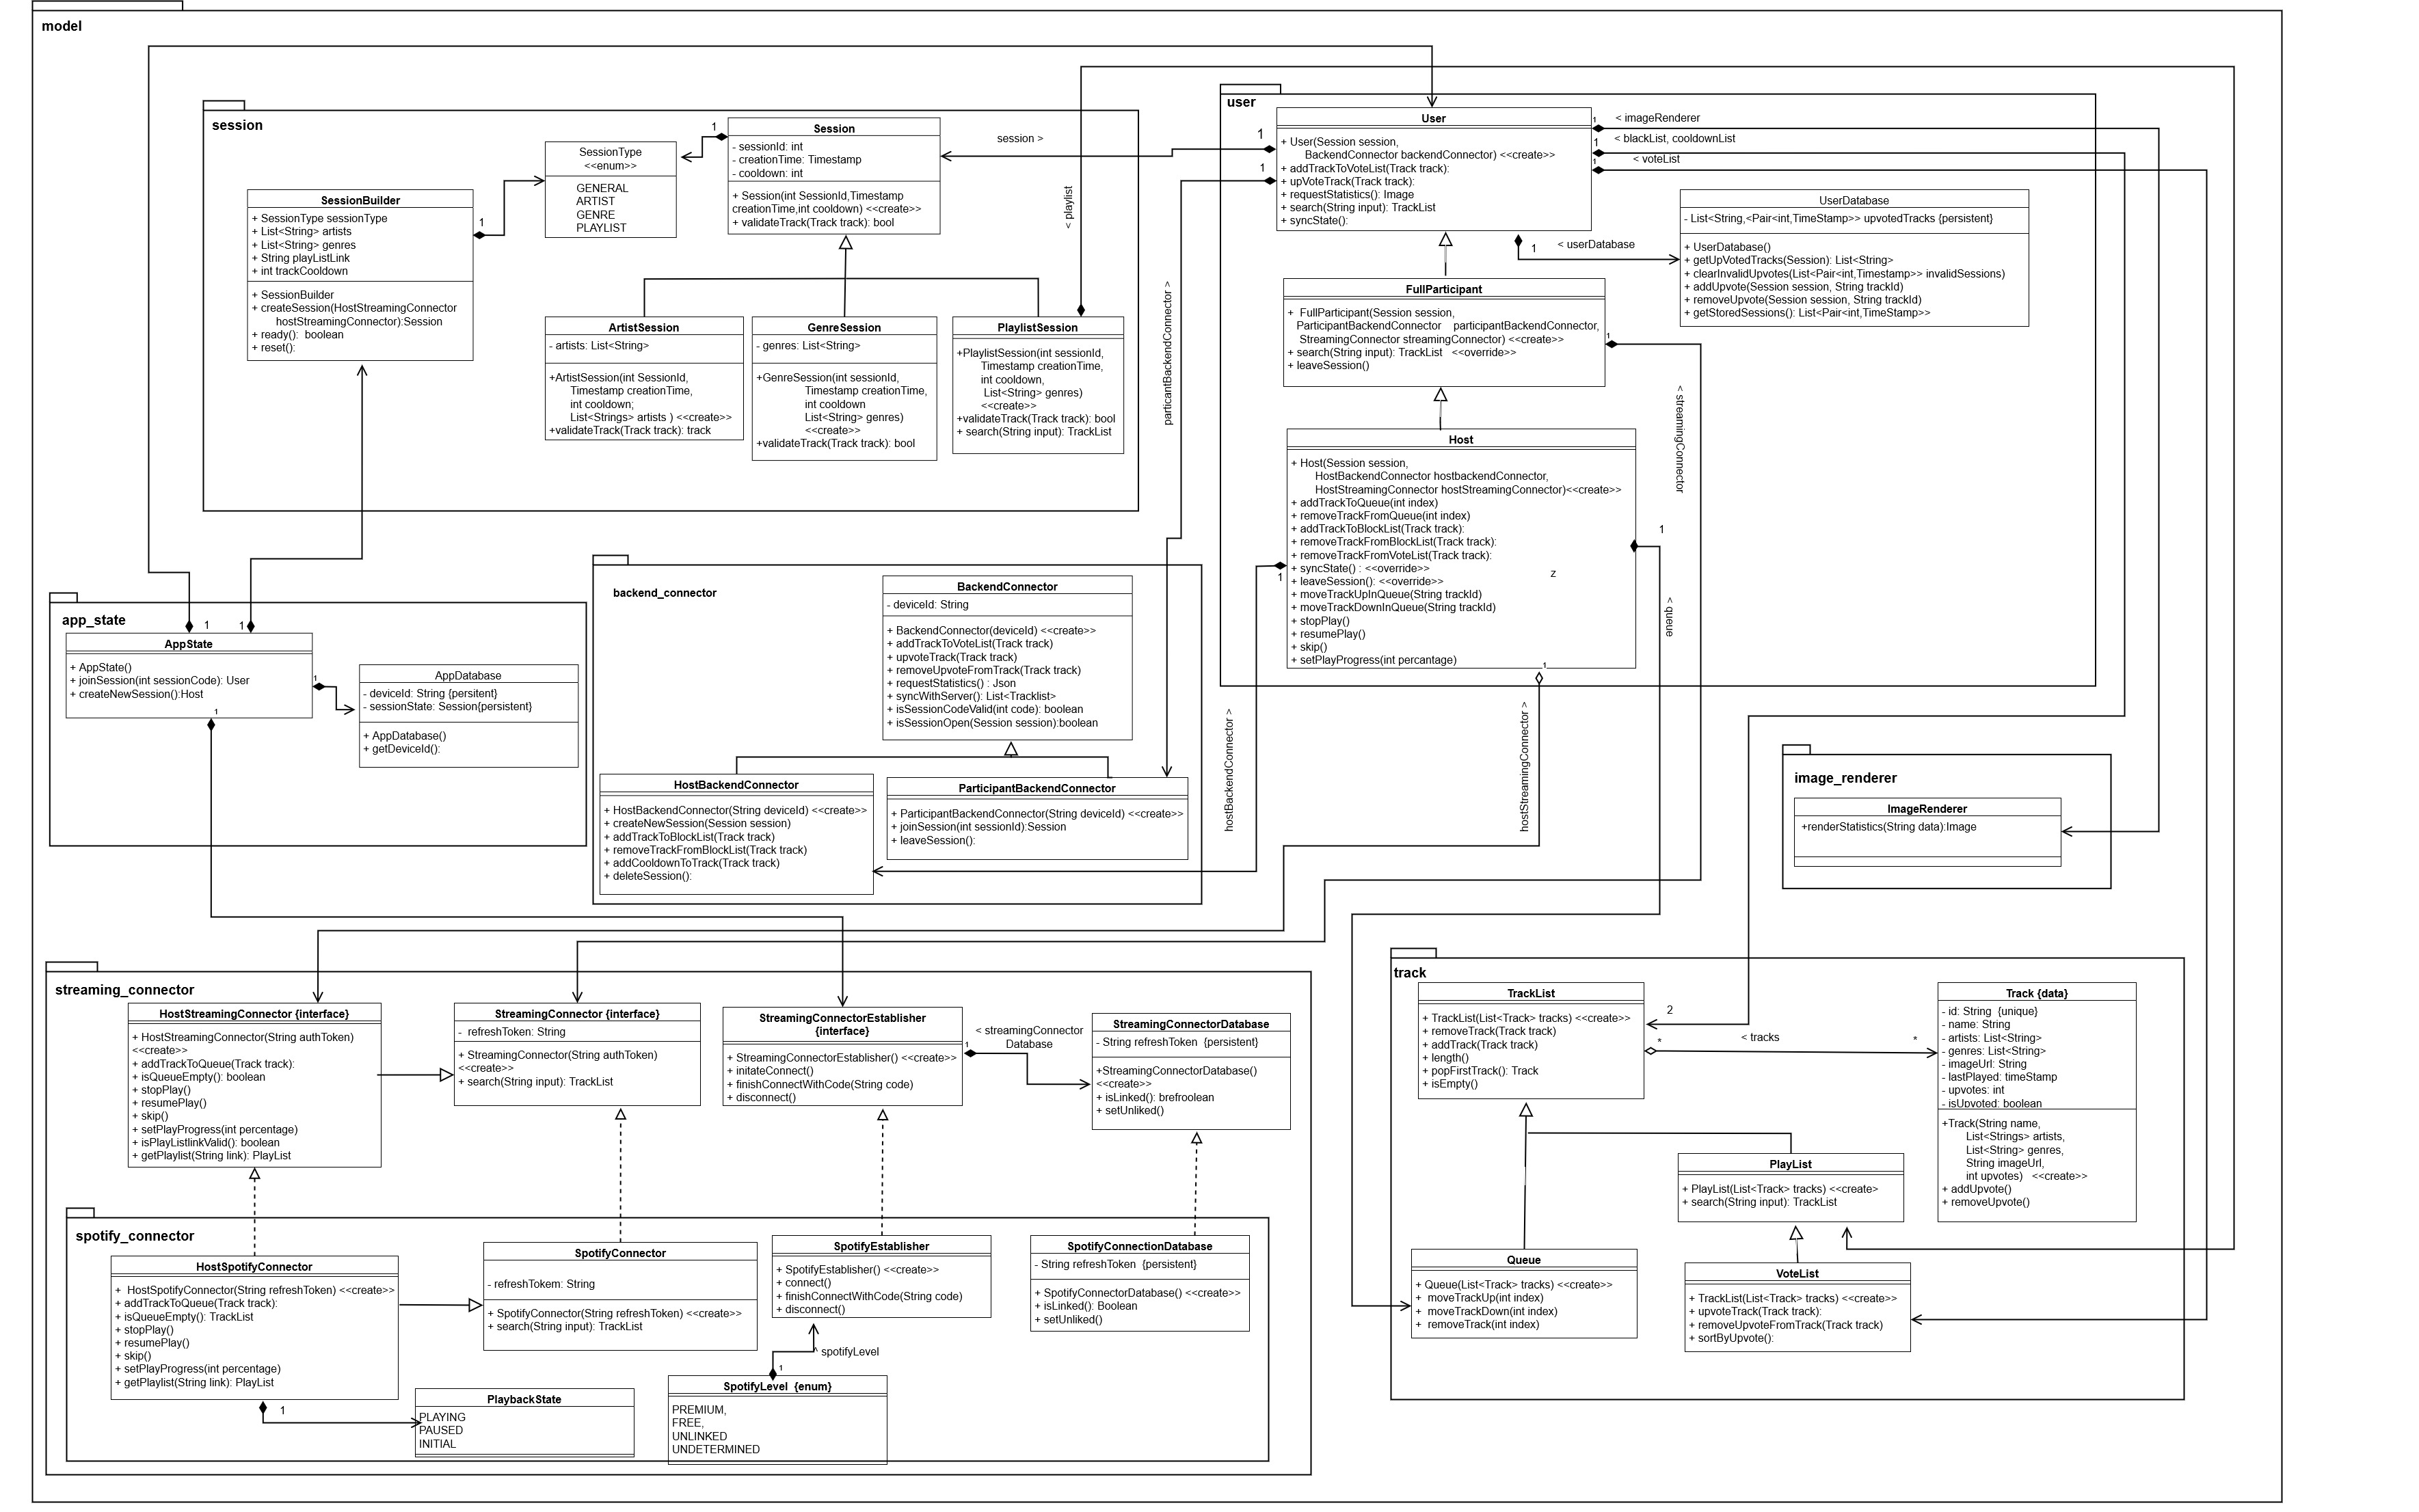
\includegraphics[width = 25cm,angle = 90]{LATEX/Entwurf/Graphics/model(6).jpg}
\captionof{figure}{model uml-diagramm}
\subsection{session}
\label{sec:App:Model:SessionPacket}
\begin{center}
   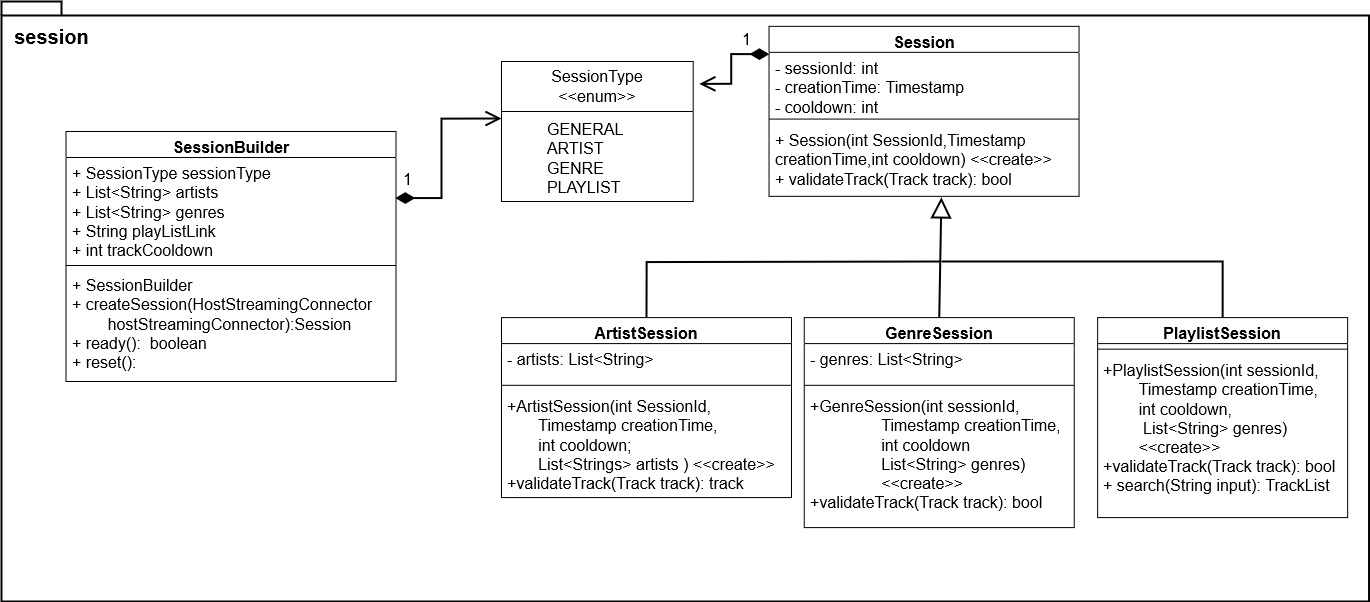
\includegraphics[width = 16cm]{LATEX/Entwurf/Graphics/session.jpg} 
\end{center}
\captionof{figure}{session uml-diagramm}

Holds all the data associated with a session, inheritance is used to implement different types of sessions and their unique requirements.
\subsubsection{Enum SessionType}

Enum to differentiate between the different SessionTypes.

\textbf{values}:
\begin{itemize}
    \item GENERAL
    \item ARTIST
    \item GENRE
    \item PLAYLIST
\end{itemize}

\subsubsection{class: Session}
Represents a Session in General Mode. Acts as a parent class for the further sessiontype classes.

\textbf{attributes:}
\begin{itemize}
    \item private: sessionId: int        
    \item private: creationTime: Timestamp
    \begin{itemize}
        \item sessionId and timestamp in combination are unique, and can be used as a unique identifer for sessions.
    \end{itemize}
    \item private: cooldownType: int
    \begin{itemize}
        \item the time in minutes a Track is on cooldown for after having been played.
    \end{itemize}
    \item public final sessionType: SessionType
\end{itemize}

\textbf{constructors:}
\begin{itemize}
    \item Session(int sessionId,Timestampt creationTime)
    \begin{itemize}
        \item assigns arguments to attributes.
        \item sets sessionType to SessionType.GENERAL
        \item \textit{implementiert <F 6.5>}
    \end{itemize}
\end{itemize}
\textbf{methods:}
\begin{itemize}
    \item getSessionId(): int
    \begin{itemize}
        \item getter for SessionId.
    \end{itemize}
    \item getTimeStamp()
    \begin{itemize}
        \item getter for TimeStamp.
    \end{itemize}
    \item getCooldown()
    \begin{itemize}
        \item getter for cooldown.
    \end{itemize}
    \item validateTrack(Track track): bool 
    \begin{itemize}
        \item checks if the track is restricted by sessionType.  
        \item returns if True by default, child classes override this method to add restrictions.
    \end{itemize}
    
\end{itemize}

\subsubsection{class: ArtistSession}
Inherits from Session, represents a Session in Artist mode.

\textbf{attributes:}
\begin{itemize}
    \item private artists: List<String>
    \begin{itemize}
        \item list of all artists allowed in the session.
    \end{itemize}
\end{itemize}
\textbf{constructors:}
\begin{itemize}
    \item ArtistSession(int SessionId,TimeStamp timestamp,List<String> artists)
    \begin{itemize}
        \item assigns arguments to attributes.
        \item sets sessionType to SessionType.ARTIST
        \item \textit{implementiert <F 6.5>}
    \end{itemize}
\end{itemize}

\textbf{methods:}
\begin{itemize}
    \item validateTrack(Track track):bool
    \begin{itemize}
        \item returns True, if the artist of the track is included in artists, false otherwise
    \end{itemize}
\end{itemize}

\subsubsection{class: GenreSession}
Inherits from Session, represents a Session in Genremode.

\textbf{attributes:}
\begin{itemize}
    \item private genre: List<String>
    \begin{itemize}
        \item list of all genres allowed in the session.
    \end{itemize}
\end{itemize}
\textbf{constructors:}
\begin{itemize}
    \item GenreSession(int SessionId,TimeStamp timestamp,List<String> genres)
    \begin{itemize}
        \item assigns arguments to attributes.
        \item sets sessionType to SessionType.GENRE
        \item \textit{implementiert <F 6.5>}
    \end{itemize}
\end{itemize}

\textbf{methods:}
\begin{itemize}
    \item validateTrack(Track track):bool
    \begin{itemize}
        \item returns True, if the genre of the track is included in genres, false otherwise
    \end{itemize}
\end{itemize}

\subsubsection{Class PlaylistSession}
Inherits from Session, represents a Session in Playlistmode.

\textbf{attributes:}
\begin{itemize}
    \item private playlist: PlayList
    \begin{itemize}
        \item list of all tracks allowed in the session.
    \end{itemize}
\end{itemize}
\textbf{constructors:}
\begin{itemize}
    \item PlayListSession(int SessionId,TimeStamp timestamp,List<String> artists)
    \begin{itemize}
        \item assigns arguments to attributes.
        \item sets sessionType to SessionType.PLAYLIST
        \item \textit{implementiert <F 6.5>}
    \end{itemize}
\end{itemize}

\textbf{methods:}
\begin{itemize}
    \item validateTrack(Track track):bool
    \begin{itemize}
        \item returns True, if the track is included in tracklist, false otherwise.
    \end{itemize}
    \item search(String input): Tracklist
    \begin{itemize}
        \item search the tracks in playlist with playlist.search(input).
        \item Returns found Tracks as TrackList
    \end{itemize}
\end{itemize}

\subsubsection{class: SessionBuilder}
The SessionBuilder collects all the data required to create a session instance and verifies it.

\textbf{attributes:}
\begin{itemize}
    \item private sessionType: SessionType
    \begin{itemize}
        \item enum indicates the Type of Session
    \end{itemize}
    \item private artists: List<String>
    \begin{itemize}
        \item list of all artists permitted in the session, null if not in ArtistMode
    \end{itemize}
    \item private genres: List<String>
    \begin{itemize}
        \item list of all genres permitted in the session, null if not in ArtistMode
    \end{itemize}
    \item private playListLink: String
    \begin{itemize}
        \item the link to the the Spotify-PlayList, null if not in PlaylistMode
    \end{itemize}
    \item private trackCooldown: int
    \begin{itemize}
        \item the cooldown of a track after it has been played in minutes
    \end{itemize}
\end{itemize}
\textbf{constructors:}
\begin{itemize}
    \item SessionBuidler()
    \begin{itemize}
        \item sets the sessionType to SessionType.GENERAL and the trackCooldown to 60min.
        \item all other attributes remain NULL.
    \end{itemize}
\end{itemize}
\textbf{methods:}
\begin{itemize}
    \item setSessionType(SessionType sessionType):
    \begin{itemize}
        \item setter for SessionType.
    \end{itemize}
    \item setArtists(List<String> artists):
    \begin{itemize}
        \item setter for artists
        \item \textit{implementiert <F 11.2>}
    \end{itemize}
     \item setGenres(List<String> genres):
    \begin{itemize}
        \item setter for genres.
        \item \textit{implementiert <F 12.2>}
    \end{itemize}
     \item setPlaylistLink(String playListLink):
    \begin{itemize}
        \item setter for playListLink.
        \item \textit{implementiert <F 6.1>}
    \end{itemize}
    \item createSession(HostStreamingConnector hostStreamingConnector)
    \begin{itemize}
        \item if the sessionType is PLAYLIST use hostStreamingConnector.getPlaylist(playListLink) to get the playList form the streaming-provider.
        \item create a Session according to the sessionType and return it, for example if sessionType = GENRE, create a GenreSession. 
    \end{itemize}
    \item ready(): boolean
    \begin{itemize}
        \item checks whether the state of the attributes is ready to build  session-instance from it. 
    \end{itemize}
    \item reset()
    \begin{itemize}
        \item sets the attributes artists, genres and playListLink back to NULL.
    \end{itemize}
\end{itemize}


\subsection{backend\_connector}
\begin{center}
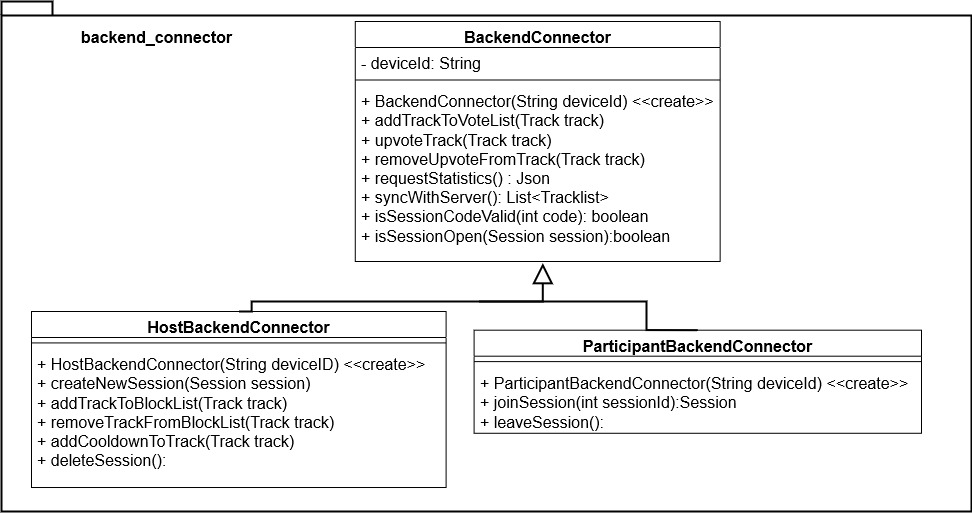
\includegraphics[width = 16cm]{LATEX/Entwurf/Graphics/BackendConnector(3).jpg}
\end{center}
\captionof{figure}{backend\_connector  uml-diagramm}
Wraps all access to the backend into one package. Depending on the role of the user, different extensions to the base BackendConnector are added using inheritance. 



 \subsubsection{class: BackendConnector}
 This class provides the base functionality for communicating with the backend for all types of users.

 \textbf{attributes:}
 \begin{itemize}
     \item private final deviceId: String 
 \end{itemize}
 \textbf{constructors:}
 \begin{itemize}
     \item BackendConnector(String deviceId):
     \begin{itemize}
         \item assigns deviceId to attribute.
     \end{itemize}
 \end{itemize}
 \textbf{methods:}
 \begin{itemize}
     \item addTrackToVoteList(Track track) 
     \begin{itemize}
         \item post deviceId and track.Id to https://nep-tune.de:5000/addNewTrack
         \item throws BackendError if returned status is ''failed''
     \end{itemize}
     \item upvoteTrack(Track track)
     \begin{itemize}
         \item post deviceId and track.Id to https://nep-tune.de:5000/addUpvoteToTrack
         \item throws BackendError if returned status is ''failed''
     \end{itemize}
     \item removeUpvoteFromTrack(Track track)
     \begin{itemize}
         \item post deviceId and track.Id to https://nep-tune.de:5000/removeUpvoteFromTrack
          \item throws BackendError if returned status is ''failed''
     \end{itemize}
     \item requestStatistics()
     \begin{itemize}
         \item post deviceID to https://nep-tune.de:5000/getStatatistics
         \item return the jsonresponse from the backend to the caller for further processing
         \item throws BackendError if returned status is ''failed''
     \end{itemize}
     
     \item syncWithServer():
     \begin{itemize}
         \item post deviceId and https://nep-tune.de:5000/getAllTrackData
         \item extract Votelist, BlackList and Cooldownlist from server response, and 
         return them in a List of Tracklists 
         \item throws BackendError if returned status is ''failed''
     \end{itemize}
     \item isSessionCodeValid(int code):bool
     \begin{itemize}
         \item \ post session.sessionId to https://nep-tune.de:5000/isSessionCodeValid
         \item parse and return response as boolean
     \end{itemize}
     \item isSessionOpen(int sessionId, TimeStamp timeStamp): bool
     \begin{itemize}
         \item post deviceId, session.sessionId and session.timestamp to https://nep-tune.de:5000/isSessionOpen
         \item parses backendresponse and returns isOpen field. 
         \item throws BackendError if returned status is ''failed'' 
     \end{itemize}
 \end{itemize}

 \subsubsection{Class ParticantBackendConnector}
Inherits from BackendConnector, adds methods needed by users in the participant role.

\textbf{attributes:}
\begin{itemize}
     \item none
\end{itemize}
\textbf{constructors:}
\begin{itemize}
    \item ParticipantBackendConnector(String deviceId)
    \begin{itemize}
        \item call super(deviceId) to invoke BackendConnector(String deviceId).
    \end{itemize}
\end{itemize}
\textbf{methods:}
\begin{itemize}
    \item joinSession(int sessionId): Session
    \begin{itemize}
          \item post deviceId and sessionId to https://nep-tune.de:5000/particantJoinSession
          \item parse the server response into a Session instance that gets returned to the caller.
         \item throws BackendError if returned status is ''failed''
     \end{itemize}
     \item leaveSession():
     \begin{itemize}
         \item post deviceId to https://nep-tune.de:5000/participantLeaveSession
         \item throws BackendError if returned status is ''failed''
     \end{itemize}
\end{itemize}

\subsubsection{class: HostBackendConnector}
Inherits from BackendConnector, adds methods needed by users in the host role.

\textbf{attributes:}
\begin{itemize}
     \item none
\end{itemize}
\textbf{constructors:}
\begin{itemize}
    \item HostBackendConnector(String deviceId)
    \begin{itemize}
        \item call super(deviceId) to invoce BackendConnector(String deviceId)
    \end{itemize}
\end{itemize}
\textbf{methods:}
\begin{itemize}
    \item createNewSession(Session session):
    \begin{itemize}
        \item post deviceId and session data to https://nep-tune.de:5000/createNewSession.
        \item sets session.creationTime to the timestamp returned from the server.
        \item throws BackendError if returned status is ''failed''.
    \end{itemize}
    \item addTrackToBlockList(Track track):
    \begin{itemize}
        \item post deviceId and track.ID with ''blocked'' = true to https://nep-tune.de:5000/setBlockTrack.
        \item throws BackendError if returned status is ''failed''.
    \end{itemize}
    \item removeTrackFromBlockList(Track track):
    \begin{itemize}
        \item post deviceId and track.ID  with ''blocked'' = false to https://nep-tune.de:5000/setBlockTrack
        \item throws BackendError if returned status is ''failed''.
    \end{itemize}
    \item addCooldownToTrack(Track track)
    \begin{itemize}
        \item post deviceId and track.ID  to https://nep-tune.de:5000/playedTrack
        \item throws BackendError if returned status is ''failed''.
    \end{itemize}
    \item deleteSession()
    \begin{itemize}
        \item post deviceId to https://nep-tune.de:5000/deleteSession
        \item throws BackendError if returned status is ''failed''.
    \end{itemize}
\end{itemize}

\subsection{track}
This packet implements different kinds of lists of tracks depending on their use case.

\begin{center}
   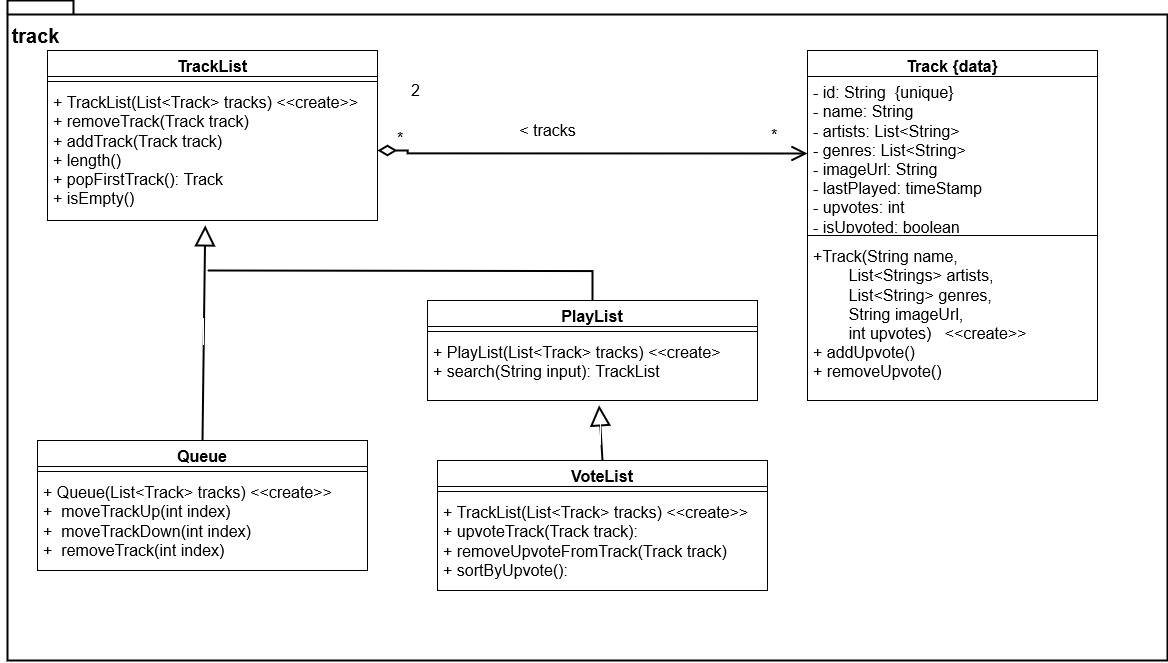
\includegraphics[width = 16cm]{LATEX/Entwurf/Graphics/track(3).jpg} 
\end{center}

\captionof{figure}{track uml-diagramm}

\subsubsection{class: Track}
Holds all data associated with a Track and provides methods to change the upvote count.

\textbf{attributes:}
\begin{itemize}
    \item private id: String {unique}
    \begin{itemize}
        \item unique id from music streaming provider.
    \end{itemize}
    \item private name: String
    \begin{itemize}
        \item name that is displayed to the user.
    \end{itemize}
    \item private artists: List<String>
    \begin{itemize}
        \item list of all artists associated with this track.
    \end{itemize}
    \item private genres: List<String>
    \begin{itemize}
         \item list of all genres associated with this track.
    \end{itemize}
    \item private imageUrl: String
    \begin{itemize}
        \item url of the image belonging to the track.
    \end{itemize}
    \item private lastPlayed: timeStamp
    \begin{itemize}
        \item Timestamp of the last time the track was played.
        \item Zero, if the track hasn´t been played yet.
    \end{itemize}
    \item private isUpvoted: boolean
    \begin{itemize}
        \item true if the track is currently upvoted by the current user, false otherwise.
    \end{itemize}
\end{itemize}
\textbf{constructors:}
\begin{itemize}
    \item Track(String name,List<Strings> artists,List<String> genres,String imageUrl,int upvotes)
    \begin{itemize}
        \item assign all the arguments to the attributes.
    \end{itemize}
\end{itemize}
\textbf{methods:}
\begin{itemize}
    \item getId(): int
    \begin{itemize}
        \item getter for id.
    \end{itemize}
    \item getName(): String
    \begin{itemize}
        \item getter for name.
    \end{itemize}
    \item getGenres(): List<String>
    \begin{itemize}
        \item getter for genres.
    \end{itemize}
    \item getterImageUrl(): String
    \begin{itemize}
        \item getter for the imageUrl
    \end{itemize}
    \item getLastPlayed(): TimeStamp
    \begin{itemize}
        \item getter for lastPlayed.
    \end{itemize}
    \item getIsUpvoted(): boolean
    \begin{itemize}
        \item getter for isUpvoted.
    \end{itemize}
    \item setIsUpvoted(boolean isUpvoted):
    \begin{itemize}
        \item setter for isUpvoted
    \end{itemize}
    \item setLastPlayed(TimeStamp playTime):
    \begin{itemize}
        \item setter for lastPlayed.
    \end{itemize}
    \item addUpvote()
    \begin{itemize}
        \item adds one to upvote counter.
    \end{itemize}
    \item removeUpvote()
    \begin{itemize}
        \item subtracts one from the upvote counter.
    \end{itemize}
    
\end{itemize}

\subsubsection{class: TrackList}
\textbf{attributes:}
\begin{itemize}
    \item tracks: List<Track>
\end{itemize}

\textbf{constructors:}
\begin{itemize}
    \item TrackList(List<Track> tracks) 
    \begin{itemize}
        \item assign argument to the attribute.
    \end{itemize}
\end{itemize}

\textbf{methods:}
\begin{itemize}
    \item getTracks()
\end{itemize}
    \begin{itemize}
        \item getter for tracks.
    \end{itemize}
    \begin{itemize}
    \item removeTrack(Track track)
    \begin{itemize}
        \item removes the track from this.tracks.
    \end{itemize}
    \item addTrack(Track track)
    \begin{itemize}
        \item add the track to this.tracks at the last position.
    \end{itemize}
    \item containsTrack(Track track)
    \begin{itemize}
        \item returns True if track is in this.tracks, False otherwise.
    \end{itemize}
    
    \item length()
    \begin{itemize}
        \item returns the amount of tracks in the TrackList.
    \end{itemize}
    \item popFirstTrack(): Track
    \begin{itemize}
        \item removes the first track from tracks and returns it. 
    \end{itemize}
    \item getTracks()
    \begin{itemize}
        \item getter for tracks.
    \end{itemize}
    
\end{itemize}

\subsubsection{class: Queue}
Inherits from TrackList, adds methods specific to the queue.

\textbf{attributes:}
\begin{itemize}
    \item None
\end{itemize}
\textbf{constructors:}
\begin{itemize}
    \item Queue(List<Track> tracks)
    \begin{itemize}
        \item call super(tracks).
    \end{itemize}
\end{itemize}
\textbf{methods:}
\begin{itemize}
    \item moveTrackDown(int  index)
    \begin{itemize}
        \item moves the track at the index one position down.
        \item if the index is in the last position nothing happens.
    \end{itemize}
    \item moveTrackUp(int index)
    \begin{itemize}
        \item moves the track at the index one position up.
        \item if the track is in the first position nothing happens.
    \end{itemize}
\end{itemize}

\subsubsection{class: PlayList}
Inherits from TrackList, adds methods specific to a playlist.

\textbf{attributes:}
\begin{itemize}
    \item None
\end{itemize}
\textbf{constructors:}
\begin{itemize}
    \item PlayList(List<Track> tracks)
    \begin{itemize}
        \item call super(tracks)
    \end{itemize}
\end{itemize}
\textbf{methods:}
\begin{itemize}
    \item search(String input): TrackList
    \begin{itemize}
        \item finds the tracks with the closest names to the input String and returns them as a TrackList.
    \end{itemize}
\end{itemize}
\subsubsection{class: VoteList}
Inherits from PlayList , adds methods specific to a VoteList.

\textbf{attributes:}
\begin{itemize}
    \item None
\end{itemize}
\textbf{constructors:}
\begin{itemize}
    \item VoteList(List<Track> tracks)
    \begin{itemize}
        \item call super(tracks)
    \end{itemize}
\end{itemize}
\textbf{methods:}
\begin{itemize}
    \item upvoteTrack(Track track):
    \begin{itemize}
        \item finds the track with the corresponding Id in tracks and adds an upvote to it.
    \end{itemize}
    \item removeUpvoteFromTrack(Track track):
    \begin{itemize}
        \item finds the track with the corresponding Id in tracks and removes an upvote from it.
    \end{itemize}
    \item sortByUpvote()
    \begin{itemize}
        \item sorts the TrackList by the amount of upvotes of the tracks.
    \end{itemize}
\end{itemize}

\subsection{streaming\_connector}
\begin{center}
   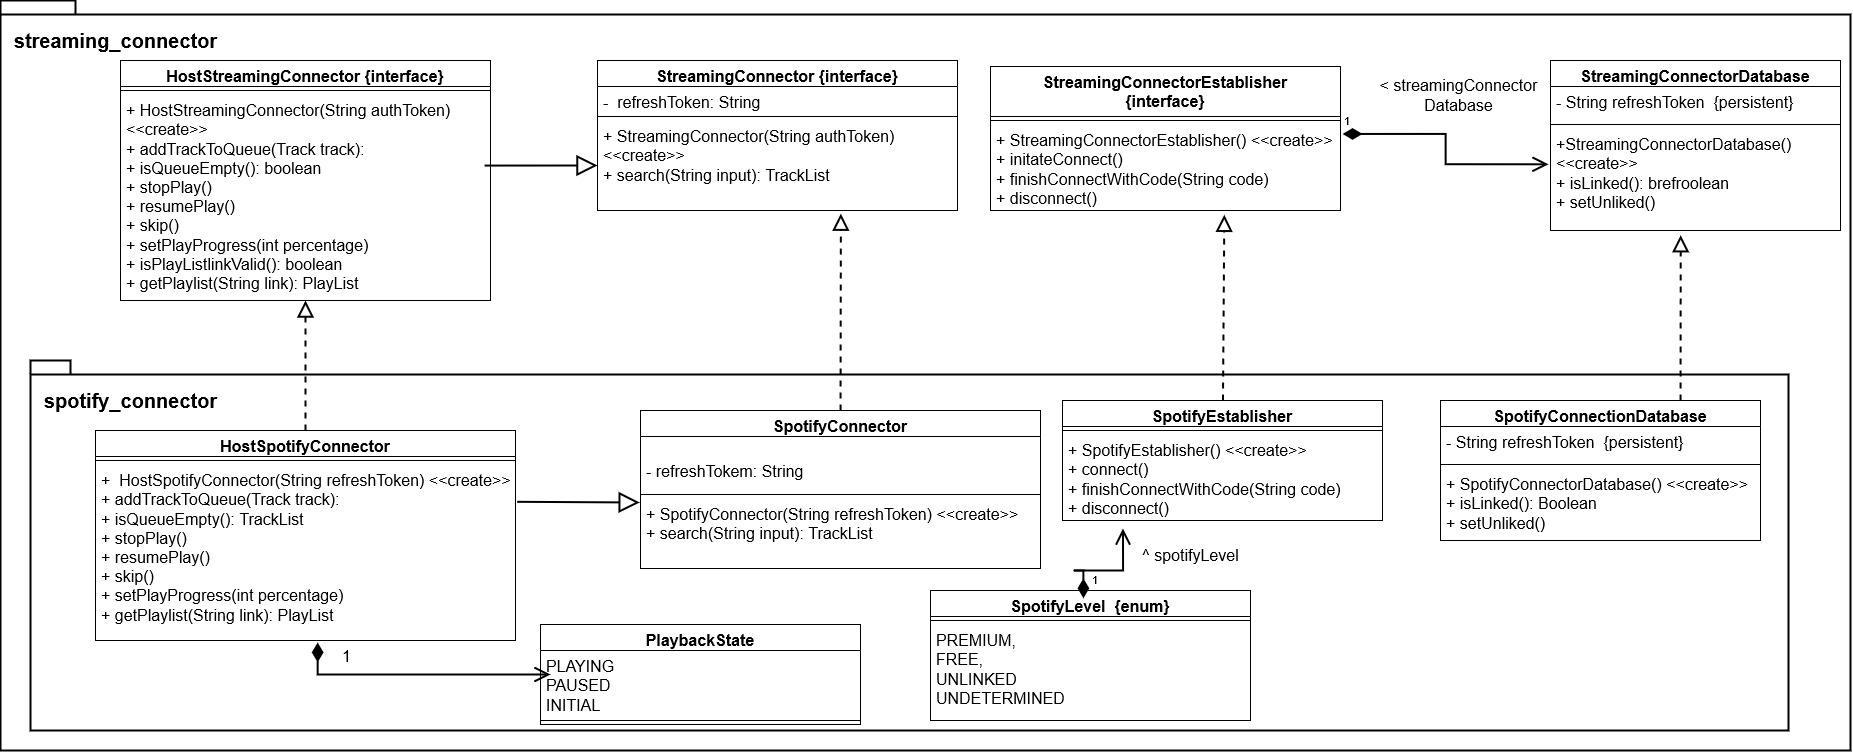
\includegraphics[width = 16cm]{LATEX/Entwurf/Graphics/streaming_connector.jpg} 
\end{center}
\captionof{figure}{session uml-diagramm}
This package defines a common interface for the connection to a music streaming provider

\subsubsection{interface: StreamingConnector}
This interface defines the base functionality necessary for every user. 

\textbf{attributes:}
\begin{itemize}
    \item refreshToken: String
    \begin{itemize}
        \item token to authenticate the user for api calls.
    \end{itemize}
    
\end{itemize}
\textbf{constructor:}
\begin{itemize}
    \item StreamingConnector(String refreshToken)
    \begin{itemize}
        \item assign arguments to refreshToken.
    \end{itemize}
\end{itemize}
\textbf{methods:}
\begin{itemize}
    \item search(String input): TrackList
    \begin{itemize}
        \item makes an api call to the music streaming provider, compiles a TrackList from the result and return it. 
    \end{itemize}
\end{itemize}

\subsubsection{interface: HostStreamingConnector}
This interface inherits from the StreamingConnector-interface and extends it with the methods needed for the Host role. 

\textbf{attributes:}
\begin{itemize}
    \item none
\end{itemize}
\textbf{constructor:}
\begin{itemize}
    \item HostStreamingConnector(String refreshToken)
    \begin{itemize}
        \item calls super(refreshToken).
    \end{itemize}
\end{itemize}
\textbf{methods:}
\begin{itemize}
    \item addTrackToQueue(Track track)
    \begin{itemize}
        \item adds the track to the music streaming provider queue using an API call
    \end{itemize}
    \item isQueueEmpty(): boolean
    \begin{itemize}
        \item Performs an API call to Spotify to check whether the queue of the music streaming provider is empty.
        \item returns True if the queue is empty, False otherwise
    \end{itemize}
    \item stopPlay()
    \begin{itemize}
        \item Performs an API call to Spotify to stop playing the current song.
    \end{itemize}
    \item resumePlay()
    \begin{itemize}
        \item Performs an API call to Spotify to resume playing the currently stopped song.
    \end{itemize}
    \item skip()
    \begin{itemize}
        \item makes an API-call to skip the currently playing song.
        \item call syncState() to replace the track in the queue of the streaming-provider.
    \end{itemize}
    \item setPlayProgess(int percentage)
    \begin{itemize}
        \item gets the length of the currently playing track from the streaming-provider with an API call.
        \item sets the play progress in spotify to  percentage *length with an API call.
    \end{itemize}
    \item getPlaylist(String link): PlayList
    \begin{itemize}
        \item gets the Playlist associated with the link and returns it as an instance of PlayList
    \end{itemize}
\end{itemize}

\subsubsection{interface: StreamingConnectorEstablisher}
This interface defines various methods to connect to the music streaming provider.

\textbf{attributes:}
\begin{itemize}
    \item public streamingConnector: StreamingConnectorDatabase
\end{itemize}
\textbf{constructors:}
\begin{itemize}
    \item StreamingConnectorEstabliser()
\end{itemize}
\textbf{methods:}
\begin{itemize}
    \item initiateConnect()
    \begin{itemize}
        \item opens the connection website of the music streaming provider.
        \item \textit{implementiert <F 1.3.A>}
    \end{itemize}
    \item finishConnectWithCode(String code):
    \begin{itemize}
        \item uses the code given as an input to finish the connection to the music streaming provider.
    \end{itemize}
    \item disconnect()
    \begin{itemize}
        \item disconnects the App from spotify, sets the refreshToken to Null in the database.
        \item \textit{implementiert <F 1.3.B>}
    \end{itemize}
\end{itemize}

\subsubsection{interface: StreamingConnectorDatabase}
This interface defines methods to persistently store data necessary for the connection to the music streaming provider.

\textbf{attributes:}
\begin{itemize}
    \item private refreshToken: String {persistent}
    \begin{itemize}
        \item used to create new authTokens
    \end{itemize}
\end{itemize}
\textbf{constructors:}
\begin{itemize}
    \item StreamingConnectorDatabase()
    \begin{itemize}
        \item sets the refreshToken to NULL if it hasn´t been set yet.
    \end{itemize}
\end{itemize}
\textbf{methods:}
\begin{itemize}
    \item isLinked(): boolean
    \begin{itemize}
        \item return false if refreshToken is NULL, true otherwise
    \end{itemize}
    \item getRefreshToken(): String
    \begin{itemize}
        \item getter for refreshToken.
    \end{itemize}
    \item setRefreshToken(String refreshToken)
    \begin{itemize}
        \item setter for refreshToken.
    \end{itemize}
    \item setUnliked()
    \begin{itemize}
        \item set refreshToken to NULL.
    \end{itemize}
\end{itemize}

\subsection{spotify\_connector}

Implements the interfaces defined in the streaming\_connector module for the music streaming provider Spotify

\subsubsection{class: SpotifyConnector}
Implements the interface StreamingConnector for the music streaming provider Spotify.

\textbf{attributes:}
\begin{itemize}
    \item refreshToken: String
    \begin{itemize}
        \item used to authenticate the request to spotify
    \end{itemize}
\end{itemize}
\textbf{constructor:}
\begin{itemize}
    \item SpotifyConnector(String authToken)
    \begin{itemize}
        \item assign arguments to authToken.
    \end{itemize}
\end{itemize}
\textbf{methods:}
\begin{itemize}
    \item search(String input): TrackList
    \begin{itemize}
        \item  performs an API call to spotify, compiles a TrackList from the result and returns it. 
    \end{itemize}
\end{itemize}


\subsubsection{class: HostSpotifyConnector}
This class implements the HostStreamingConnector-interface for Spotify.

\textbf{attributes:}
\begin{itemize}
    \item none
\end{itemize}
\textbf{constructor:}
\begin{itemize}
    \item HostSpotifyConnector(String refreshToken)
    \begin{itemize}
        \item calls super(refreshToken ).
    \end{itemize}
\end{itemize}
\textbf{methods:}
\begin{itemize}
    \item addTrackToQueue(Track track)
    \begin{itemize}
        \item adds the track to the music streaming provider queue with an API call
    \end{itemize}
    \item isQueueEmpty(): boolean
    \begin{itemize}
        \item Performs an API call to check whether the queue of the music streaming provider is empty.
        \item returns True if the queue is empty, false otherwise
    \end{itemize}
    \item stopPlay()
    \begin{itemize}
        \item Performs an API call to stop playing the current song
    \end{itemize}
    \item resumePlay()
    \begin{itemize}
        \item Performs an API call to start playing the currently stopped song
    \end{itemize}
    \item skip()
    \begin{itemize}
        \item Performs an API call to skip the currently playing song.
        \item call syncState() to replace the track in the queue of spotify.
    \end{itemize}
    \item setPlayProgess(int percentage)
    \begin{itemize}
        \item gets the length of the currently playing track in the music streaming provider using an API call.
        \item sets the Playprogress in music streaming provider to  percentage *length using an API call.
    \end{itemize}
    \item getPlaylist(String link): PlayList
    \begin{itemize}
        \item gets the Playlist associated with the link and returns it as an instance of PlayList
    \end{itemize}
\end{itemize}

\subsubsection{class: SpotifyConnectorEstablisher}
This class implements the StreamingConnectorEstablisher-interface for Spotify.

\textbf{attributes:}
\begin{itemize}
    \item public spotifyConnectionDatabase: SpotifyConnectionDatabase
\end{itemize}
\textbf{constructors:}
\begin{itemize}
    \item StreamingConnectorEstabliser()
\end{itemize}
\textbf{methods:}
\begin{itemize}
    \item initateConnect()
    \begin{itemize}
        \item opens the the connection-website of the music streaming provider
    \end{itemize}
    \item finishConnectWithCode(String code):
    \begin{itemize}
        \item uses the code given as an input to finish the connection to music streaming provider.
    \end{itemize}
    \item disconnect()
    \begin{itemize}
        \item disconnects the App from spotify, sets the refreshToken to Null in the database
    \end{itemize}
\end{itemize}

\subsubsection{class: SpotifyConnectorDatabase}
This class implements the StreamingConnectorDatabase-interface for Spotify.

\textbf{attributes:}
\begin{itemize}
    \item private refreshToken: String {persistent}
    \begin{itemize}
        \item used to create new authTokens for Spotify.
    \end{itemize}
\end{itemize}
\textbf{constructors:}
\begin{itemize}
    \item StreamingConnectorDatabase()
    \begin{itemize}
       \item sets the refreshToken to NULL if it hasn´t been set yet.
    \end{itemize}
\end{itemize}
\textbf{methods:}
\begin{itemize}
    \item isLinked(): boolean
    \begin{itemize}
        \item return false if refreshToken is NULL, true otherwise.
    \end{itemize}
    \item getRefreshToken(): String
    \begin{itemize}
        \item getter for refreshToken.
    \end{itemize}
    \item setRefreshToken(String refreshToken)
    \begin{itemize}
        \item setter for refreshToken.
    \end{itemize}
    \item setUnliked()
    \begin{itemize}
        \item set refreshToken to NULL.
    \end{itemize}
\end{itemize}

\subsubsection{enum: SpotifyLevel}
Enum of all possible connection states concerning Spotify.

\textbf{values:}
\begin{itemize}
    \item PREMIUM
    \item FREE
    \item UNLINKED
    \item UNDETERMIND
\end{itemize}

\subsection{image\_renderer}
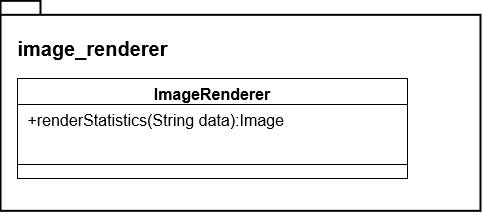
\includegraphics[width = 14 cm]{LATEX/Entwurf/Graphics/image_renderer(1).jpg}
\captionof{figure}{image\_renderer uml diagramm}
\subsubsection{class: ImageRenderer}
The ImageRenderer receives data and renders an image containing session statistics, ready to be displayed to the user.

\textbf{attributes}:
\begin{itemize}
    \item none
\end{itemize}
\textbf{constructors:}
\begin{itemize}
    \item default
\end{itemize}
\textbf{methods:}
\begin{itemize}
    \item renderStatistics(String json): Image
    \begin{itemize}
        \item parses the json to get the relevant data.
        \item renders an image, containing the data and returns it.
    \end{itemize}
\end{itemize} 


\subsection{user}

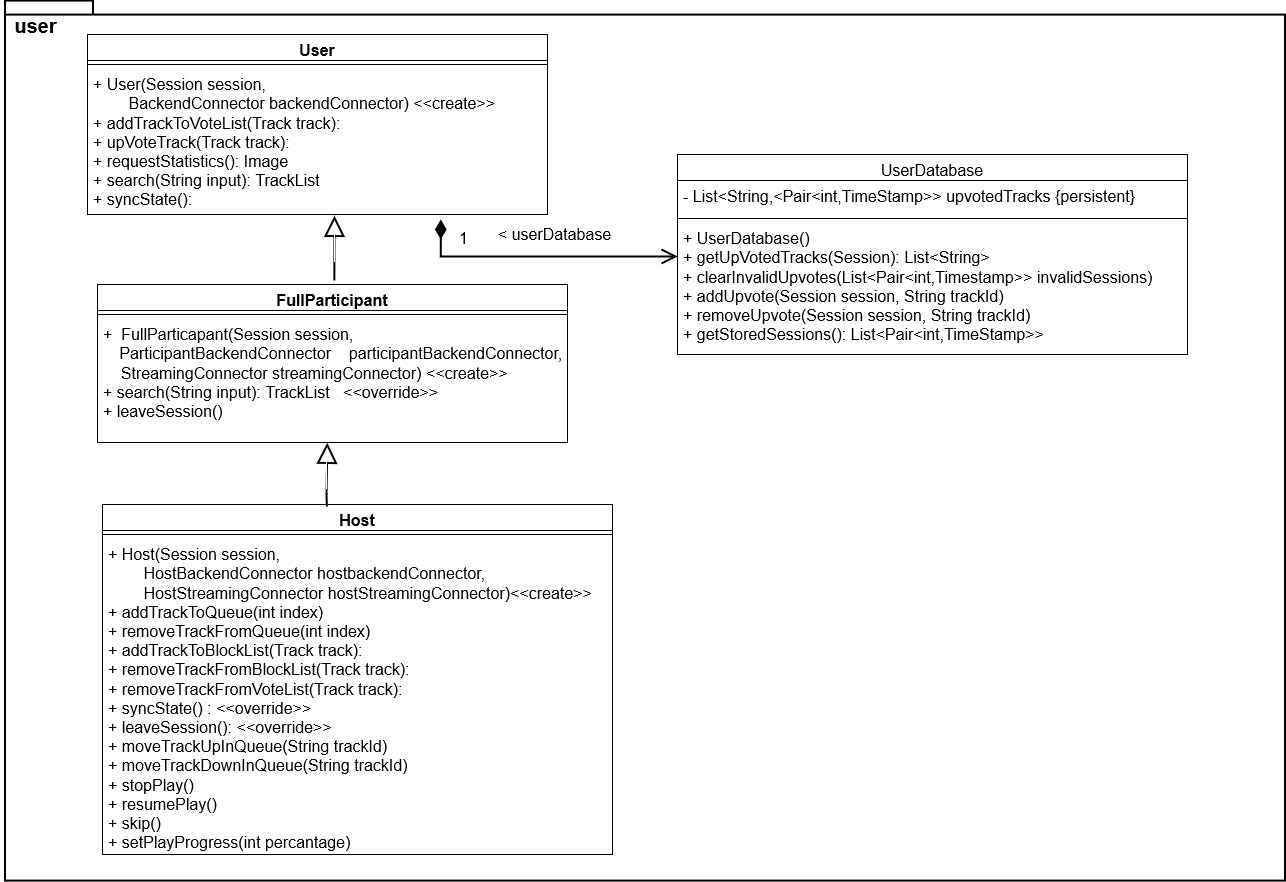
\includegraphics[width = 16 cm]{LATEX/Entwurf/Graphics/user(1).jpg}
\captionof{figure}{user uml diagramm}
The User class and its child classes act as a facade between the ViewModel and the Model. All user interaction after the creation of a session goes through the user, the user object updates its inner state accordingly and uses the BackendConnector to communicate changes to the Server.
The syncState-method should be called in regular intervalls to sync with the Backend. This synchronization includes the updating of the upvote counter and adds the tracks having been added by different users. 


\subsubsection{class: User}
Implements core functionality necessary for all Users regardless of their role.
Instances of this class represent, a user in the restricted particant role.
\textbf{attributes:}
\begin{itemize}
    \item private userDatabase: UserDatabase
    \begin{itemize}
        \item Persistently stores the tracks the user has upvoted in a session .
    \end{itemize}
    \item private  voteList: VoteList 
    \begin{itemize}
        \item list of all tracks which can be voted on currently
        \item sorted by upvotes 
    \end{itemize}
    \item private blockList: TrackList
    \begin{itemize}
        \item list of all tracks that are currently blacklisted.
    \end{itemize}
    \item private cooldownList: TrackList
    \begin{itemize}
        \item list of all tracks that are currently on cooldown.
    \end{itemize}
    \item private imageRenderer: imageRenderer
    \begin{itemize}
        \item imageRenderer handles the rendering of the statistics image.
    \end{itemize}
\end{itemize}
\textbf{constructors:}
\begin{itemize}
    \item User(Session session, BackendConnector backendConnector)
    \begin{itemize}
        \item assigns arguments to attributes.
        \item create empty VoteList and assign it to voteList.
        \item create two TrackLists and assign them to blocklist and cooldownList.
        \item create ImageRender instance and assign it to the matching attribute. 
        \item clear the UserDatabase from invalid entries, this step involves:
        \begin{itemize}
            \item create UserDataBase-instance and assign it to the userDataBase-attribute.
            \item call userDataBase.getStoredSessions() to get all Sessions with entries in the database.
            \item use backendConnector.isSessionOpen(sessionId,timeStamp) to check which sessions are still valid. 
            \item call userDatabase.clearInvalidUpvotes with a list of all the invalid upvotes.
        \end{itemize}
    \end{itemize}
\end{itemize}
\textbf{methods:}
\begin{itemize}
    \item addTrackToVoteList(Track track)
    \begin{itemize}
        \item add track to VoteList
        \item calls backendConnector.addTrackToVoteList(track) to add track in the backend.
    \end{itemize}
    \item upvoteTrack(Track track):
    \begin{itemize}
        \item calls voteList.upvoteTrack(track)
        \item calls backendConnector.addTrackToVoteList(track) to add upvote in the backend.
        \item \textit{implementiert <F 3.3.A>, <F 4.4.A>, <F 7.3.A>, <7.6.A>}
    \end{itemize}
    \item removeVoteFromTrack(Track track):
        \begin{itemize}
            \item calls voteList.removeUpvoteFromTrack(track)
            \item calls backendConnector.removeUpvoteFromTrack(track) to remove upvote in the backend.
            \item \textit{implementiert <F 3.3.B>, <F 4.4.B>, <F 7.3.B>, <7.6.B>}
        \end{itemize}
    \item search(String input):
    \begin{itemize}
        \item finds the tracks with the most similiar names to the input and returns them in a TrackList.
        \item \textit{implementiert <F 4.3>, <F 8.3>}
    \end{itemize}
    \item requestStatistics()
    \begin{itemize}
      \item calls backendConnector.requestStatistics() to receive the necessary data as a Json-String from the backend.
      \item pass data on to imageRender.renderStatisitics to get an image.
      \item return the resulting image.
    \end{itemize}
    \item syncState():
    \begin{itemize}
        \item calls backendConnector.syncwithServer() and assigns the returned trackLists to the voteList, cooldownList and blackList
        \item sort the voteList with voteList.sortByUpvote()
        \item after this method the state of user is in sync with the backend.
    \end{itemize}
    
\end{itemize}

\subsubsection{class FullParticant:}
Inherits from User, and adds methods specific to the FullParticipant role.

\textbf{attributes}
\begin{itemize}
    \item none
\end{itemize}
\textbf{constructors:}
\begin{itemize}
\item FullParticipant(Session session,ParticipantBackendConnector participantBackendConnector,StreamingConnector streamingConnector) 
\end{itemize}
\begin{itemize}
    \item call super(session,participantBackendConnector,streamingConnector)
    \item participantBackendConnector gets cast to instance of BackendConnector, but can be casted back to ParticipantBackendConnector if required.
\end{itemize}
\textbf{methods}:
\begin{itemize}
    \item search(String input):
    \begin{itemize}
        \item searches the input in the VoteList and with spotifyConnector.search(input).
        \item validates that found tracks are not restricted by the session with session.validateTrack(track).
        \item returns the found tracks as TrackList.
    \end{itemize}
    \item leaveSession():
    \begin{itemize}
        \item cast backendConnector back to particantBackendConnector()
        \item call particantBackendConnector.leaveSession()
    \end{itemize}
    
\end{itemize}




\subsubsection{class Host:}
Inherits from FullParticipant, and adds methods specific to the Host role. 

\textbf{attributes:}
\begin{itemize}
    \item private queue: Queue
    \begin{itemize}
        \item list of all tracks currently in the queue to be played next.
    \end{itemize}
\end{itemize}
\textbf{constructors:}
\begin{itemize}
    \item Host(Session session, BackendConnector backendConnector, HostStreamingConnector hostStreamingConnector)
    \begin{itemize}
        \item calls super(session, hostBackendConnector,hostStreamingConnector).
        \item The hostBackendConnector gets cast to BackendConnector, but can be cast back to HostBackendConnector instance at any time.
        \item The hostBackendConnector gets cast to StreamingConnector, but can be cast back to HostStreamingConnector-instance at any time.
    \end{itemize}
\end{itemize}
\textbf{methods:}
\begin{itemize}
    \item addTrackToQueue(Track track)
    \begin{itemize}
        \item adds track to this.queue at the last position.
        \item \textit{implementiert <F 7.7.A>, <F 8.5.A>}
    \end{itemize}
    \item removeTrackFromQueue(Track track)
    \begin{itemize}
        \item remove track from this.queue.
        \item \textit{implementiert <F 7.4.A>}
    \end{itemize}
    \item addTrackToBlockList(Track track):
    \begin{itemize}
        \item adds track to this.blockList
        \item casts the backendConnector back to an hostBackendConnector
        \item call hostBackendConnector.addTrackToBlockList(track) to mark the track as blocked in the backend.
        \item \textit{implementiert <F 7.4.B>, <7.7.B>, <8.5.B>}
    \end{itemize}
    \item removeTrackFromBlockList(Track track):
    \begin{itemize}
        \item remove track from this.blockList
        \item casts the backendConnector back to an hostBackendConnector
        \item call removeTrackFromBlockList(track) to mark the track as not blocked anymore in the backend.
    \end{itemize}
    \item syncState(): <<override>>
    \begin{itemize}
        \item call super.syncState().
        \item casts streamingConnector back to hostStreamingConnector
        \item cast backendConnector back to hostBackendConnector
        \item calls hostStreamingConnector.isQueueEmpty() to check whether the queue of the streaming provider is empty. If the queue of the streaming provider is empty, add the first track in the queue with an API call to the streaming provider queue. If the queue is empty,  add the highest upvoted track from the voteList instead.
        \item set the cooldown of the added track, and use hostBackendConnector.addCooldownToTrack(track) to set the Cooldown of the Track in the backend.
        \end{itemize}
    \item leaveSession() <<override>>
    \begin{itemize}
        \item casts the backendConnector back to a hostBackendConnector
        \item call hostBackendConnector.deleteSession() to delete the session in the backend. 
    \end{itemize}
    \item moveTrackUpInQueue(int index)
     \begin{itemize}
         \item calls the queue.moveTrackUp(index) to move track up in the queue
         \item \textit{implementiert <F 7.5>, <F 7.8>}
     \end{itemize}
     \item moveTrackDownInQueue(int index)
      \begin{itemize}
         \item calls the queue.moveTrackDown(trackId) to move track down in the queue
         \item \textit{implementiert <F 7.5>, <7.8>}
     \end{itemize}
     \item stopPlay()
     \begin{itemize}
         \item casts the streamingConnector back to the hostStreamingConnector.
         \item call hostStreamingConnector.stop() to stop the playback of the  track currently playing.
     \end{itemize}
     \item resumePlay()
     \begin{itemize}
         \item casts the streamingConnector back to the hostStreamingConnector.
         \item call hostStreamingConnector.resume() to stop the playback of the current playing track.
     \end{itemize}
     \item setPlayProgress(int percentage)
     \begin{itemize}
         \item casts the streamingConnector back to the hostStreamingConnector.
         \item call hostStreamingConnector.setPlayProgress(progress) to set play progress of the currently playing track.
     \end{itemize}
\end{itemize}

\subsubsection{class: UserDataBase}
This class stores and manages the persistent data associated with each user-instance.

\textbf{attributes:}
\begin{itemize}
    \item private upvotedTracks: List<String,Pair<int,TimeStamp>> \{persistent\}
    \begin{itemize}
        \item stores the SessionId for every trackId  and the creation time of the session, if the Track was upvoted by this User in this session.
    \end{itemize}
\end{itemize}
\textbf{constructors:}
\begin{itemize}
    \item default
\end{itemize}
\textbf{methods:}
\begin{itemize}
    \item getUpvotedTracks(Session session): List<String>
    \begin{itemize}
        \item return the trackId of all the tracks the user has upvoted in the session supplied as an argument.
    \end{itemize}
    \item clearInvalidUpvotes(List<Pair<int,Timestamp>> invalidSessions)
    \begin{itemize}
        \item deletes all entries associated with the invalid session from upvotedTracks
    \end{itemize}
    \item addUpvote(Session session, String trackId)
    \begin{itemize}
        \item adds an entry to the upvotedTracks:
    \end{itemize}
    \item removeUpvote(Session session, String trackId)
    \begin{itemize}
        \item removes the entry from upvotedTracks.
    \end{itemize}
    \item getStoredSessions(): List<Pair<int,TimeStamp>>
    \begin{itemize}
        \item returns a list of all the sessionIds and timestamps of the sessions with upvoted tracks in the Database.
    \end{itemize}
\end{itemize}

\subsection{app\_state}


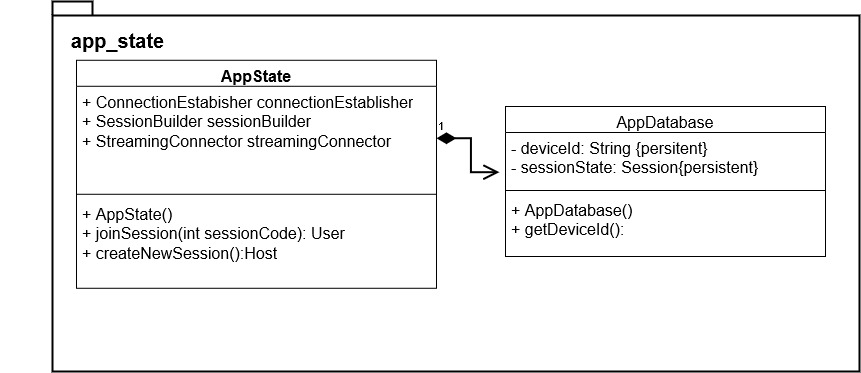
\includegraphics[width = 14 cm]{LATEX/Entwurf/Graphics/app_state.jpg}
\captionof{figure}{app\_state uml diagramm}

\subsubsection{class: AppState}
The AppState class manages all relevant data, till the user enters a session.

\textbf{attributes:}
\begin{itemize}
    \item public connectionEstablisher: ConnectionEstablisher
    \begin{itemize}
        \item connects and disconnects from Spotify.
    \end{itemize}
    \item public sessionBuilder: SessionBuilder
    \begin{itemize}
        \item collects all the data neccesary to construct an instance of Session.
    \end{itemize}
\end{itemize}

\textbf{constructors:}
\begin{itemize}
    \item AppState()
    \begin{itemize}
        \item construct connectionEstablisher and assign it to the attribute.
        \item construct sessionBuilder and assign it to the attribute.
    \end{itemize}
    
\end{itemize}

\textbf{methods:}
\begin{itemize}
    \item joinSession(int sessionCode): User
    \begin{itemize}
        \item the front end makes sure that the button which calls join Session is only active if the sessionCode is valid, therefore the function only gets called with valid sessionCode.
        \item create ParticantBackendConnector instance and call joinSession(sessionCode) to get a session-instance from the back end 
        \item save the Session in appDatabase with saveSession-method.
        \item look up the SpotifyLevel in the streamerConnectorDatabase, if the Level is UNLINKED create a User-instance and return it, otherwise initialize a SpotifyConnector-instance and create a FullParticipant-instance
        and return it.
        
    \end{itemize}
    \item createNewSession(): Host
    \begin{itemize}
        \item create instance of HostSpotifyConnector
        \item call sessionBuilder.createSession(hostSpotifyConnector) to get a session instance.
        \item save the Session in appDatabase with saveSession-method.
        \item create HostBackendConnnector instance and use the createNewSession-method to register the new session with the back end.
        \item create a Host-instance and return it.
    \end{itemize}
\end{itemize}

\subsubsection{class: AppDatabase}
Stores the relevant data necessary for authenticating the user with the back end and restoring a session after the app has been shut down.

\textbf{attributes:}
\begin{itemize}
    \item private final deviceId: String {persistent}
    \begin{itemize}
        \item used to authenticate the device with the back end.
    \end{itemize}
    \item private sessionState: Session {persistent}
    \begin{itemize}
        \item Persistently stores the currently active session. This enables restoring a session after the app has been shut down.
    \end{itemize}
\end{itemize}
\textbf{constructors:}
\begin{itemize}
    \item AppDataBase()
    \begin{itemize}
        \item if deviceId is not assigned, generate deviceId and store it persistently.
    \end{itemize}
\end{itemize}
\textbf{methods:}
\begin{itemize}
    \item getDeviceId(): String
    \begin{itemize}
        \item getter for SessionId
    \end{itemize}
    \item saveSession(Session session)
    \begin{itemize}
        \item stores the current session-instance persistently in the appDatabase.
    \end{itemize}
    \item getSession(): Session
    \begin{itemize}
        \item getter for the stored session-instance.
    \end{itemize}
\end{itemize}







\section{UI}
\label{sec:App:UI}

Alle Klassen und Funktionen des UI (User Interface) befinden sich in einem eigenen Paket ui, das auf höchster Projektebene liegt.

Vom UI umgesetzte funktionale Anforderungen:

\begin{itemize}
    \item <F 1>: StartView und StartViewModel
    \item <F 2>: JoinView und JoinViewModel
    \item <F 3>: VoteView und VoteViewModel
    \item <F 4>: SearchView und SearchViewModel
    \item <F 5>: ModeSelectView und ModeSelectViewModel
    \item <F 6>: ModeSettingsView und ModeSettingsViewModel
    \item <F 7>: ControlView und ControlViewModel
    \item <F 8>: SearchView und SearchViewModel
    \item <F 9>: InfoView und InfoViewModel
    \item <F 10>: StatsView und StatsViewModel
    \item <F 11>: EntitySelectView und EntitySelectViewModel
    \item <F 12>: EntitySelectView und EntitySelectViewModel
\end{itemize}


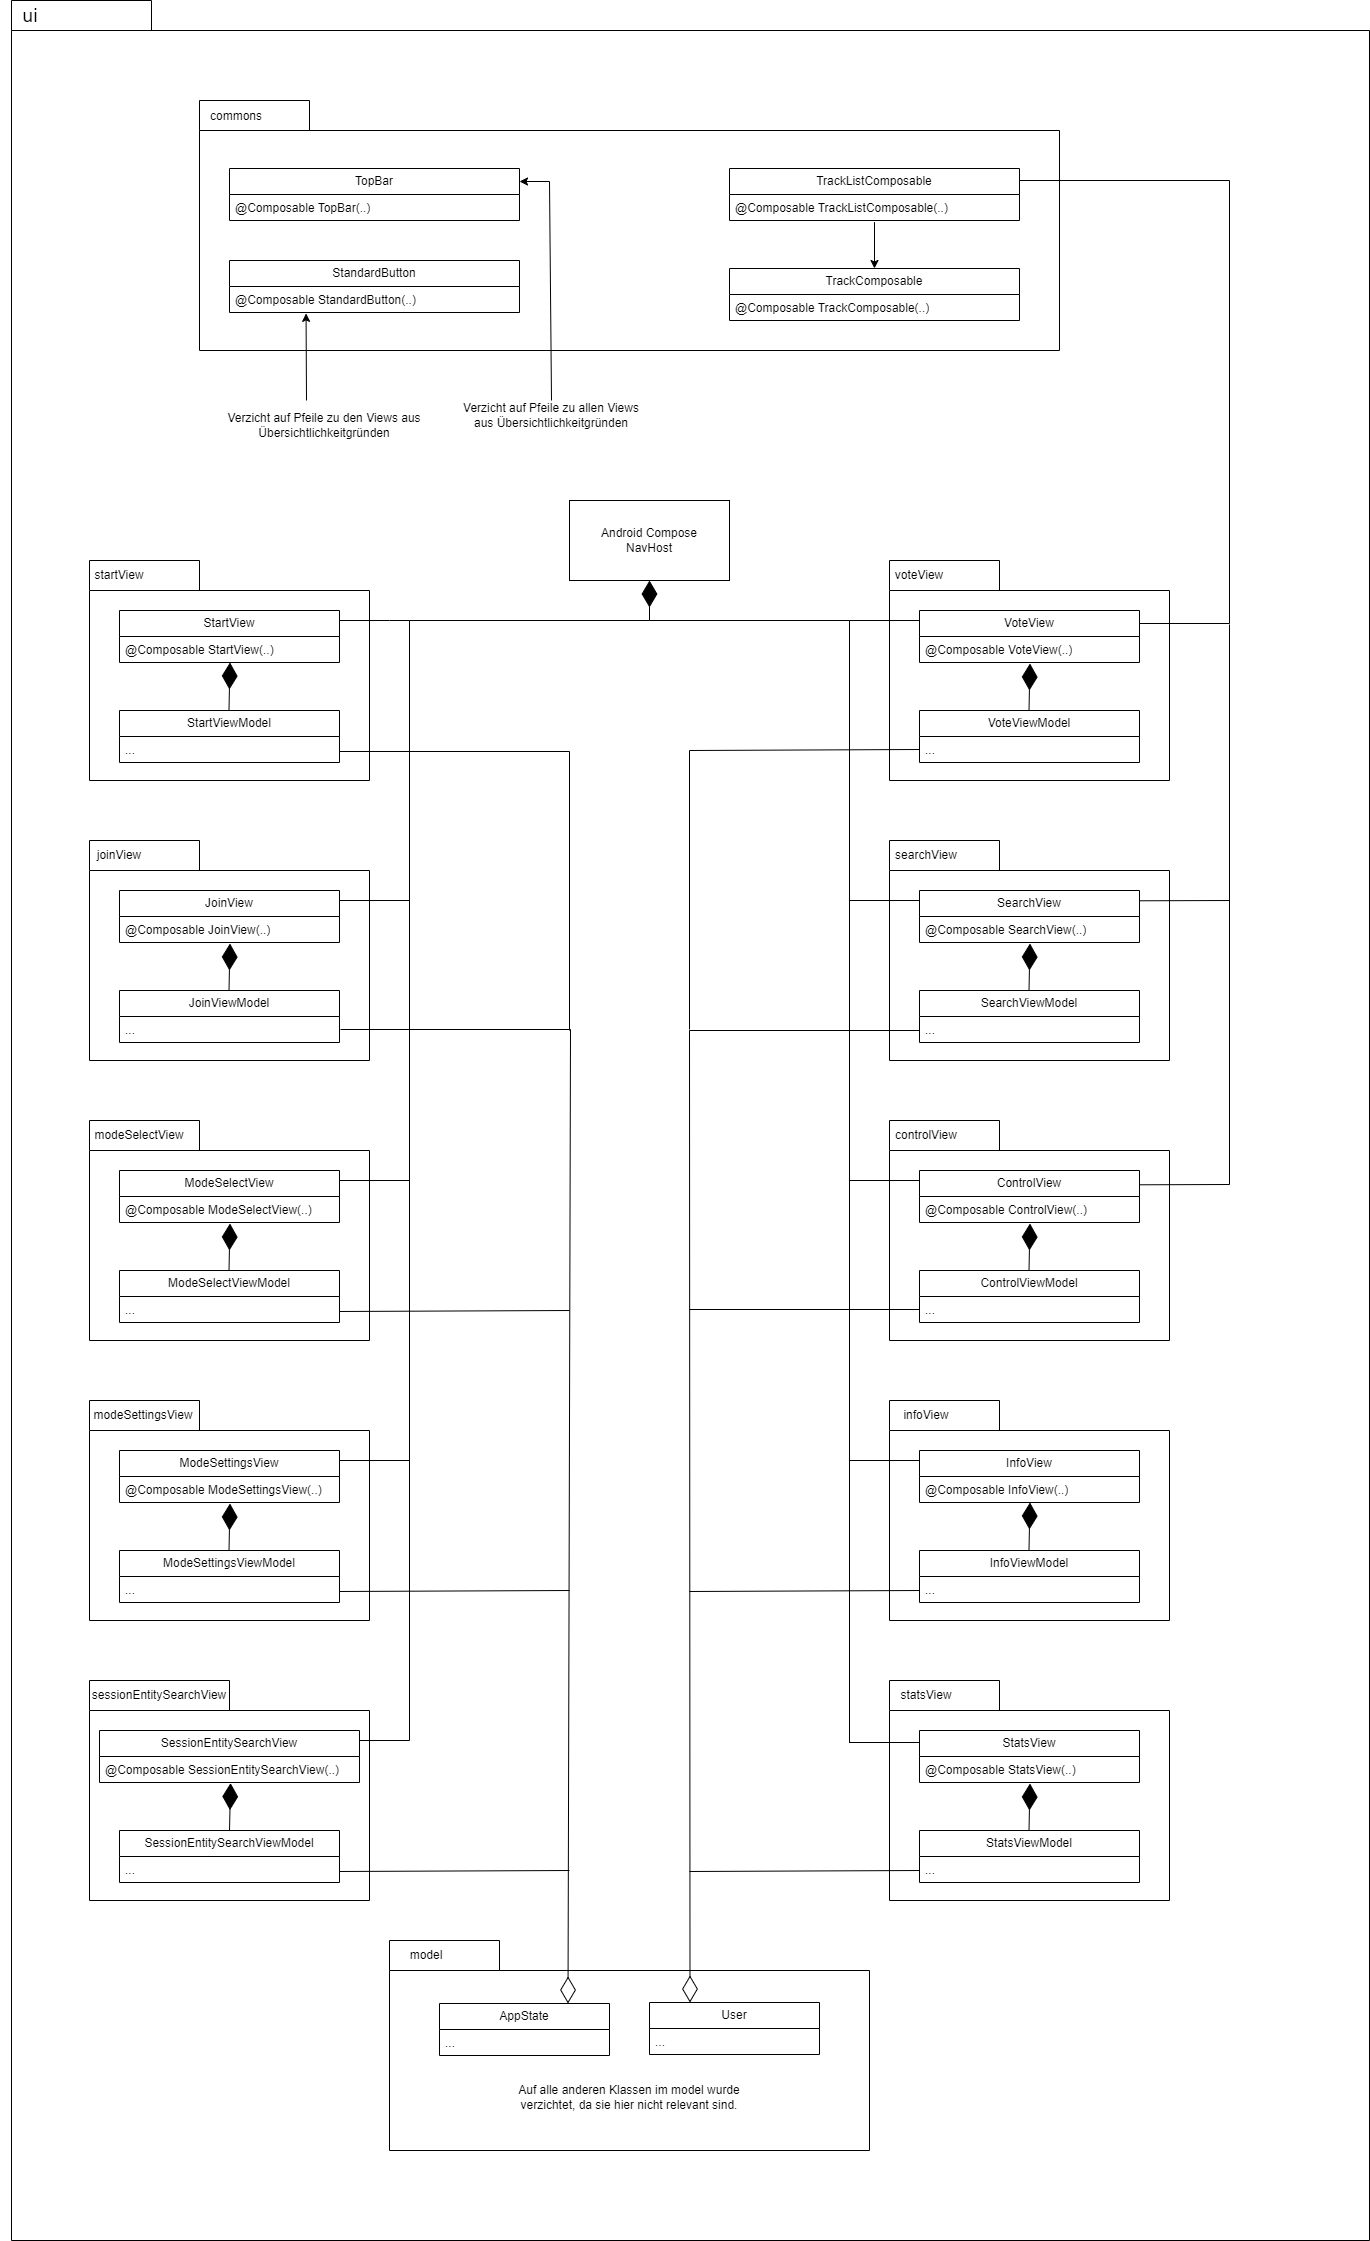
\includegraphics[width=14cm]{LATEX/Entwurf/Graphics/UI_Entwurf.png}
\captionof{figure}{UI UML-Diagramm}


\subsection{View}
\label{sec:App:View}


\subsubsection{Composable View Funktionen}
Alle Views sind mit @Composable annotierte Funktionen, die nicht explizit zu einer Klasse gehören. Jede View hat ihre eigene Datei, in der genau eine öffentliche Funktion zum Rendern der View bereitgestellt wird. All diese Views werden dem Android Compose NavHost übergeben, der die Views dann verwaltet. Jede solche Datei liegt gemeinsam mit ihrem ViewModel in einem eigenen Paket. Zur Navigation haben die Funktionen den NavController als Argument. Zusätzlich gibt es private Hilfsmethoden zum Rendern.

Dementsprechend gibt es folgende Dateien mit folgenden Funktionen in folgenden Paketen:
\begin{itemize}
    \item startView.kt \newline mit @Composable StartView(NavController navController) \newline
    im Paket ui.startView
    \item joinView.kt \newline mit @Composable JoinView(NavController navController) \newline
    im Paket ui.joinView
    \item voteView.kt \newline mit @Composable VoteView(NavController navController) \newline
    im Paket ui.voteView
    \item searchView.kt \newline mit @Composable SearchView(NavController navController) \newline
    im Paket ui.searchView
    \item modeSelectView.kt \newline mit @Composable ModeSelectView(NavController navController) \newline
    im Paket ui.modeSelectView
    \item modeSettingsView.kt \newline mit @Composable ModeSettingsView(NavController navController) \newline
    im Paket ui.modeSettingsView
    \item controlView.kt \newline mit @Composable ControlView(NavController navController) \newline
    im Paket ui.controlView
    \item infoView.kt \newline mit @Composable InfoView(NavController navController) \newline
    im Paket ui.infoView
    \item statsView.kt \newline mit @Composable StatsView(NavController navController) \newline
    im Paket ui.statsView
    \item sessionEntitiesSearchView.kt \newline mit @Composable SessionEntitiesSearchView(NavController navController) \newline
    im Paket ui.sessionEntitiesSearchView
\end{itemize}


\subsection{Composable Funktionen von häufigen UI-Elementen}

Als häufig wiederkehrende UI-Elemente haben wir die Top-Bar, die Anzeige einer Track-Liste, die Anzeige für einen einzelnen Track und den Standard-Button identifiziert. Für diese stellen wir im Paket ui.commons mit @Composable annotierte Funktionen zum Rendern bereit. Diese können von den Views aufgerufen werden, welche solche Elemente anzeigen.

\subsubsection{fun: TopBarComposable}

Hat folgende Signatur und Funktionalität:
\begin{itemize}
    \item @Composable TopBar(lambda () -> Unit onClickBack, String description)
    \begin{itemize}
        \item Shows the top bar with the app name and logo and the description.
        \item onClickBack: lamda to be called when the back button was pressed.
        \item description: Content of the top bar description, if empty no description will be shown.
    \end{itemize}
\end{itemize}


\subsubsection{fun: TrackListComposable}

Hat folgende Signatur und Funktionalität:
\begin{itemize}
    \item @Composable TrackListComposable(List<Track> tracks, TrackListType trackListType, and a lot of lambdas described in TrackComposable)
    \begin{itemize}
        \item Renders a track list with the given tracks.
        \item tracks: All the tracks to be rendered in the list.
        \item trackListType: enum of the track list type, determining the possibilities for interaction with the track.
    \end{itemize}
\end{itemize}


\subsubsection{fun: TrackComposable}

Hat folgende Signatur und Funktionalität:
\begin{itemize}
    \item @Composable TrackComposable(Track track, Int trackIndexInList, TrackListType trackListType, and a lot of lambdas described underneath)
    \begin{itemize}
        \item Renders a track given the specifications of the track list type.
        \item track: The track to be rendered.
        \item trackIndexInList: The position of the track in the track list as its index.
        \item trackListType: enum of the track list type, determining the possibilities for interaction with the track.
        \item lambda (Track) -> Unit onToggleUpvote: called when the user clicks on the upvote button, passing the track.
        \item lambda(Int) -> Unit onToggleDropdown: called when the expands or collapses the dropdown menu, passing the index of track
        \item lambda (Int) -> Boolean isDropdownExpanded: called to determine whether the dropdown menu is expanded,  passing the index of the track.
        \item lambda (Track) -> Unit onAddToQueue: called when the user clicks on adding the track to the queue, passing the track.
        \item lambda (Int) -> Unit onRemoveFromQueue: called when the user clicks on removing the track from the queue, passing the index.
        \item lambda (Track) -> Unit onToggleBlock: called when the user blocks or unblocks a track, passing the track.
        \item lambda (Int) -> Unit onMoveUp: called when the user moves a track up (in the queue), passing the index of the track.
        \item lambda (Int) -> Unit onMoveDown: called when the user moves a track down (in the queue), passing the index of the track.
    \end{itemize}
\end{itemize}


\subsubsection{fun: TrackListComposable}

Hat folgende Signatur und Funktionalität:
\begin{itemize}
    \item @Composable StandardButton(lambda () -> Unit onClick, String text, Boolean enabled, Modifier modifier)
    \begin{itemize}
        \item Renders a standard enabled or disabled button with a text description.
        \item onClick: the lambda to be called when clicked.
        \item text: the text description of the button.
        \item enabled: Whether the button is enabled and can be clicked, or disabled and cannot be clicked, affects the design of the button.
        \item modifier: Additional modifier options to be added to the button design.
    \end{itemize}
\end{itemize}




\subsection{ViewModel}
\label{sec:App:ViewModel}

Jede der Body Funktionen einer View besitzt ein ViewModel in Form einer Klasse. Diese ViewModels stellen Methoden bereit, um im UI auftretende Logik zu handlen oder Informationen mit dem Model auszutauschen. So wird sichergestellt, dass in den composable Funktionen der Views keine Logik ausgeführt wird, sondern nur deklarativ das UI definiert wird.

Alle ViewModels liegen mit den jeweiligen Composable Funktionen im selben Paket.
Jede Composable View hat eine entsprechende ViewModel Instanz.



\subsubsection{class: StartViewModel}

Benötigt folgende Attribute im Konstruktor:
\begin{itemize}
    \item AppState appState
\end{itemize}
Stellt folgende Attribute bzw. Methoden für die View bereit:
\begin{itemize}

    \item createSessionPossible(): Boolean
        \begin{itemize}
            \item Checks if it is possible to create a session, only possible if the user is a Spotify premium user.
            \item Return: Indicates the possibility of creating a session.
        \end{itemize}
    \item toggleConnectedToSpotify()
        \begin{itemize}
            \item Toggles the linked status with Spotify. Starts connecting if unlinked or disconnects otherwise.
        \end{itemize}
    \item getSpotifyButtonText(): String
        \begin{itemize}
            \item Retrieves the text for the Spotify button based on the spotify level.
            \item Return: The text for the Spotify button.
        \end{itemize}
    \item onJoinSession(NavController navController)
        \begin{itemize}
            \item Changes the view to the JoinSessionView.
            \item navController: The NavController used for navigation.
            \item \textit{implementiert <F 1.1>}
        \end{itemize}
    \item onCreateSession(NavController navController)
        \begin{itemize}
            \item Changes the view to the ModeSelectView.
            \item navController: The NavController used for navigation.
            \item \textit{implementiert <F 1.2>}
        \end{itemize}
    \item onBack(NavController navController)
        \begin{itemize}
            \item Displays the pop up window of wether to leave the app or not.
            \item navController: The NavController used for navigation.
            \item \textit{implementiert <F 1.4>}
        \end{itemize}
    \item onConfirmLeave(NavController navController)
        \begin{itemize}
            \item Closes the app when confirming to leave it.
            \item navController: The NavController used for navigation.
            \item \textit{implementiert <F 1.4.A>}
        \end{itemize}
    \item onDismissLeave(NavController navController)
        \begin{itemize}
            \item Closes the pop up window when dismissing the leave prompt.
            \item navController: The NavController used for navigation.
            \item \textit{implementiert <F 1.4.B>}
        \end{itemize}
\end{itemize}



\subsubsection{class: JoinViewModel}

Benötigt folgende Attribute im Konstruktor:
\begin{itemize}
    \item AppState appState
\end{itemize}
Stellt folgende Attribute bzw. Methoden für die View bereit:
\begin{itemize}

    \item getCodeInput(): String
        \begin{itemize}
            \item Retrieves the code input as a string.
            \item Return: The code input.
        \end{itemize}
    \item isCodeInputFormValid(): Boolean
        \begin{itemize}
            \item Checks if the code input form is valid.
            \item Return: Indicates the validity of the code input form.
        \end{itemize}
    \item onCodeInputChange(String newInput)
        \begin{itemize}
            \item Handles changes in the code input and is called when the input is updated.
            \item newInput: The new code input provided as a string.
        \end{itemize}
    \item onConfirmSessionCode(NavController navController)
        \begin{itemize}
            \item Checks the session code and changes the view to the VoteView.
            \item navController: The NavController used for navigation.
            \item \textit{implementiert <F 2.2>}
        \end{itemize}
    \item onScanQrCode()
        \begin{itemize}
            \item Initiates the process of scanning a QR code to enter the session.
            \item \textit{implementiert <F 2.3>}
        \end{itemize}
    \item onBack(NavController navController)
        \begin{itemize}
            \item Goes back to the StartView.
            \item navController: The NavController used for navigation.
            \item \textit{implementiert <F 2.5>}
        \end{itemize}
\end{itemize}



\subsubsection{class: VoteViewModel}

Benötigt folgende Attribute im Konstruktor:
\begin{itemize}
    \item User user
\end{itemize}
Stellt folgende Attribute bzw. Methoden für die View bereit:
\begin{itemize}

    \item onToggleUpvote(Track track)
        \begin{itemize}
            \item Toggles the upvote status for the given track.
            \item track: The track for which the upvote status is toggled.
        \end{itemize}
    \item onToggleDropdown(Int index)
        \begin{itemize}
            \item Toggles the dropdown menu state at the specified index in the vote list.
            \item index: The index of the dropdown to be toggled.
        \end{itemize}
    \item isDropdownExpanded(Int index): Boolean
        \begin{itemize}
            \item Checks if the dropdown menu of the track at the specified index is expanded.
            \item index: The index to be checked.
            \item Return: Indicates whether the dropdown is expanded or not.
        \end{itemize}
    \item getVoteList(): List<Track>
        \begin{itemize}
            \item Retrieves the list of tracks to be displayed in the vote list.
            \item Return: The list of tracks.
        \end{itemize}
    \item onSearchTracks(NavController navController)
        \begin{itemize}
            \item Changes the view to the track SearchView.
            \item navController: The NavController used for navigation.
            \item \textit{implementiert <F 3.4>}
        \end{itemize}
    \item getTopBarDescription(): String
        \begin{itemize}
            \item Retrieves the description for the top bar.
            \item Return: The description for the top bar.
        \end{itemize}
    \item onOpenInfo(NavController navController)
        \begin{itemize}
            \item Changes the view to the InfoView.
            \item navController: The NavController used for navigation.
            \item \textit{implementiert <F 3.1>}
        \end{itemize}
    \item onOpenStats(NavController navController)
        \begin{itemize}
            \item Changes the view to the StatsView.
            \item navController: The NavController used for navigation.
            \item \textit{implementiert <F 3.2>}
        \end{itemize}
    \item onBack(NavController navController)
        \begin{itemize}
            \item Displays the pop up window of wether to leave the session or not.
            \item navController: The NavController used for navigation.
            \item \textit{implementiert <F 3.5>}
        \end{itemize}
    \item onConfirmLeaveSession(NavController navController)
        \begin{itemize}
            \item Goes back to the StartView when confirming to leave the session.
            \item navController: The NavController used for navigation.
            \item \textit{implementiert <F 3.5.A>}
        \end{itemize}
    \item onDismissLeaveSession(NavController navController)
        \begin{itemize}
            \item Closes the pop up window when dismissing the leave prompt.
            \item navController: The NavController used for navigation.
            \item \textit{implementiert <F 3.5.B>}
        \end{itemize}
\end{itemize}



\subsubsection{class: SearchViewModel}

Benötigt folgende Attribute im Konstruktor:
\begin{itemize}
    \item User user
\end{itemize}
Stellt folgende Attribute bzw. Methoden für die View bereit:
\begin{itemize}

    \item getTrackSearchInput(): String
        \begin{itemize}
            \item Retrieves the track search input as a string.
            \item Return: The track search input.
        \end{itemize}
    \item onTrackSearchInputChange(String newInput)
        \begin{itemize}
            \item Handles changes in the track search input and is called when the input is updated.
            \item newInput: The new track search input provided as a string.
            \item \textit{implementiert <F 4.3>, <F 8.3>}
        \end{itemize}
    \item isSearchButtonActive(): Boolean
        \begin{itemize}
            \item Checks if the search button is active.
            \item Return: Indicates whether the search button is active or not.
        \end{itemize}
    \item onSearchButtonClick()
        \begin{itemize}
            \item Handles the action when the search button is clicked and then updates the search list.
        \end{itemize}
    \item onToggleUpvote(Track track)
        \begin{itemize}
            \item Toggles the upvote status for the given track.
            \item track: The track for which the upvote status is toggled.
        \end{itemize}
    \item onToggleDropdown(Int index)
        \begin{itemize}
            \item Toggles the dropdown menu state at the specified index in the vote list.
            \item index: The index of the track of which to toggle the dropdown menu.
            \item \textit{implementiert <F 8.5>}
        \end{itemize}
    \item isDropdownExpanded(Int index): Boolean
        \begin{itemize}
            \item Checks if the dropdown menu of the track at the specified index is expanded.
            \item index: The index to be checked.
            \item Return: Indicates whether the dropdown is expanded or not.
        \end{itemize}
    \item onAddToQueue(Track track)
        \begin{itemize}
            \item Adds the given track to the queue.
            \item track: The track to be added to the queue.
        \end{itemize}
    \item onToggleBlock(Track track)
        \begin{itemize}
            \item Toggles the block status for the given track.
            \item track: The track for which the block status is toggled.
        \end{itemize}
    \item getSearchList(): List<Track>
        \begin{itemize}
            \item Retrieves the list of tracks to be displayed in the search results.
            \item Return: The list of tracks.
        \end{itemize}
    \item getActiveFilter(): String
        \begin{itemize}
            \item Retrieves the currently activated filter.
            \item Return: The filter, is either none, cooldown or blocked.
        \end{itemize}
    \item onSetActiveFilter(String filter)
        \begin{itemize}
            \item Sets the active filter for the search results.
            \item filter: The filter to be set.
            \item \textit{implementiert <F 8.7>}
        \end{itemize}
    \item getCooldownTracks(): List<Track>
        \begin{itemize}
            \item Retrieves the list of tracks with cooldown to be displayed in the results.
            \item Return: The list of tracks.
            \item \textit{implementiert <F 8.7.A>}
        \end{itemize}
    \item getBlockedTracks(): List<Track>
        \begin{itemize}
            \item Retrieves the list of blocked tracks to be displayed in the results.
            \item Return: The list of tracks.
            \item \textit{implementiert <F 8.7.B>}
        \end{itemize}
    \item getTopBarDescription(): String
        \begin{itemize}
            \item Retrieves the description for the top bar.
            \item Return: The description for the top bar.
        \end{itemize}
    \item onOpenInfo(NavController navController)
        \begin{itemize}
            \item Changes the view to the InfoView.
            \item navController: The NavController used for navigation.
            \item \textit{implementiert <F 4.1>, <F 8.1>}
        \end{itemize}
    \item onOpenStats(NavController navController)
        \begin{itemize}
            \item Changes the view to the StatsView.
            \item navController: The NavController used for navigation.
            \item \textit{implementiert <F 4.2>, <8.2>}
        \end{itemize}
    \item onBack(NavController navController)
        \begin{itemize}
            \item Goes back to VoteView.
            \item navController: The NavController used for navigation.
            \item \textit{implementiert <F 4.5>, <F 8.6>}
        \end{itemize}
\end{itemize}



\subsubsection{class: ModeSelectViewModel}

Benötigt folgende Attribute im Konstruktor:
\begin{itemize}
    \item AppState appState
\end{itemize}
Stellt folgende Attribute bzw. Methoden für die View bereit:
\begin{itemize}

    \item isModeSelected(Mode mode): Boolean
    \begin{itemize}
        \item Checks if the specified mode is selected in order to display the buttons correctly.
        \item mode: The mode to be checked for selection.
        \item Return: Indicates whether the mode is selected or not.
    \end{itemize}
    \item onSelectMode(Mode mode)
        \begin{itemize}
            \item Selects the specified mode when the respective button is clicked.
            \item mode: The mode to be selected.
            \item \textit{implementiert <F 5.1.A/B/C/D>}
        \end{itemize}
    \item getSelectedModeDescription(): String
        \begin{itemize}
            \item Retrieves the description for the currently selected mode.
            \item Return: The description for the selected mode.
        \end{itemize}
    \item onConfirmMode(NavController navController)
        \begin{itemize}
            \item Goes to the ModeSettingView.
            \item navController: The NavController used for navigation.
            \item \textit{implementiert <F 5.2>}
        \end{itemize}
    \item onBack(NavController navController)
        \begin{itemize}
            \item Goes back to the StartView.
            \item navController: The NavController used for navigation.
            \item \textit{implementiert <F 5.3>}
        \end{itemize}
\end{itemize}



\subsubsection{class: ModeSettingsViewModel}

Benötigt folgende Attribute im Konstruktor:
\begin{itemize}
    \item AppState appState
\end{itemize}
Stellt folgende Attribute bzw. Methoden für die View bereit:
\begin{itemize}

    \item isPlaylistLinkInputAvailable(): Boolean
        \begin{itemize}
            \item Checks if the playlist link input is available based on the selected mode.
            \item Return: Indicates whether the playlist link input is available or not.
        \end{itemize}
    \item getPlaylistLinkInput(): String
        \begin{itemize}
            \item Retrieves the playlist link input as a string.
            \item Return: The playlist link input.
            \item \textit{implementiert <F 6.1>}
        \end{itemize}
    \item onPlaylistLinkInputChange(String newInput)
        \begin{itemize}
            \item Handles changes in the playlist link input and is called when the input is updated.
            \item newInput: The new playlist link input provided as a string.
            \item \textit{implementiert <F 6.1>}
        \end{itemize}
    \item isPlaylistLinkValid(): Boolean
        \begin{itemize}
            \item Checks if the playlist link is valid.
            \item Return: Indicates whether the playlist link is valid or not.
            \item \textit{implementiert <F 6.1>}
        \end{itemize}
    \item getCooldownSliderPosition(): Float
        \begin{itemize}
            \item Retrieves the current position of the cooldown slider.
            \item Return: The current position of the cooldown slider.
            \item \textit{implementiert <F 6.4>}
        \end{itemize}
    \item onCooldownSliderPositionChange(Float newPosition)
        \begin{itemize}
            \item Handles changes in the cooldown slider position and is called when the position is updated.
            \item newPosition: The new position of the cooldown slider provided as a float.
            \item \textit{implementiert <F 6.4>}
        \end{itemize}
    \item onCooldownSliderFinish(Float position)
        \begin{itemize}
            \item Handles the action when the cooldown slider position is not touched by the user anymore.
            \item position: The finalized position of the cooldown slider provided as a float.
            \item \textit{implementiert <F 6.4>}
        \end{itemize}
    \item getTrackCooldownString(): String
        \begin{itemize}
            \item Retrieves the string representation of the selected track cooldown.
            \item Return: The formatted string for the track cooldown.
        \end{itemize}
    \item isArtistSearchAvailable(): Boolean
        \begin{itemize}
            \item Checks if artist search is available based on the selected mode.
            \item Return: Indicates whether artist search is available or not.
        \end{itemize}
    \item onArtistSearch(NavController navController)
        \begin{itemize}
            \item Changes the view to the SessionEntitiesSearchView.
            \item navController: The NavController used for navigation.
            \item \textit{implementiert <F 6.2.A>}
        \end{itemize}
    \item getSelectedArtists(): List<String>
        \begin{itemize}
            \item Retrieves the list of selected artists.
            \item Return: The list of selected artists.
        \end{itemize}
    \item isGenreSearchAvailable(): Boolean
        \begin{itemize}
            \item Checks if genre search is available based on the selected mode.
            \item Return: Indicates whether genre search is available or not.
        \end{itemize}
    \item onGenreSearch(NavController navController)
        \begin{itemize}
            \item Changes the view to the SessionEntitiesSearchView.
            \item navController: The NavController used for navigation.
            \item \textit{implementiert <F 6.2.B>}
        \end{itemize}
    \item getSelectedGenres(): List<String>
        \begin{itemize}
            \item Retrieves the list of selected genres.
            \item Return: The list of selected genres.
        \end{itemize}
    \item onToggleSelect(String entityName)
        \begin{itemize}
            \item Toggles the selection state for the specified entity, either the artist or the genre.
            \item entityName: The name of the entity for which the selection state is toggled.
            \item \textit{implementiert <F 6.3.A>, <F 6.3.B>}
        \end{itemize}
    \item onConfirmSettings(NavController navController)
        \begin{itemize}
            \item Opens the session and goes to the ControlView.
            \item navController: The NavController used for navigation.
            \item \textit{implementiert <F 6.5>}
        \end{itemize}
    \item onBack(NavController navController)
        \begin{itemize}
            \item Goes back to the ModeSelectView.
            \item navController: The NavController used for navigation.
            \item \textit{implementiert <F 6.6>}
        \end{itemize}
\end{itemize}



\subsubsection{class: ControlViewModel}

Benötigt folgende Attribute im Konstruktor:
\begin{itemize}
    \item Host host
\end{itemize}
Stellt folgende Attribute bzw. Methoden für die View bereit:
\begin{itemize}

    \item onToggleUpvote(Track track)
        \begin{itemize}
            \item Toggles the upvote status for the given track.
            \item track: The track for which the upvote status is toggled.
        \end{itemize}
    \item onToggleDropdown(Int index)
        \begin{itemize}
            \item Toggles the dropdown menu state for the track at the specified index in the track list.
            \item index: The index of the dropdown menu to be toggled.
        \end{itemize}
    \item isDropdownExpanded(Int index): Boolean
        \begin{itemize}
            \item Checks if the dropdown menu of the track at the specified index is expanded.
            \item index: The index to be checked.
            \item Return: Indicates whether the dropdown is expanded or not.
        \end{itemize}
    \item onAddToQueue(Track track)
        \begin{itemize}
            \item Adds the given track to the queue.
            \item track: The track to be added to the queue.
        \end{itemize}
    \item onRemoveFromQueue(Int index)
        \begin{itemize}
            \item Removes the track at the specified index from the queue.
            \item index: The index of the track to be removed.
        \end{itemize}
    \item onToggleBlock(Track track)
        \begin{itemize}
            \item Toggles the block status for the given track.
            \item track: The track for which the block status is toggled.
        \end{itemize}
    \item onMoveUp(Int index)
        \begin{itemize}
            \item Moves the track at the specified index up in the queue by one spot if possible.
            \item index: The index of the track to be moved.
        \end{itemize}
    \item onMoveDown(Int index)
        \begin{itemize}
            \item Moves the track at the specified index down in the queue by one spot if possible.
            \item index: The index of the track to be moved.
        \end{itemize}
    \item getPausedDescription(): String
        \begin{itemize}
            \item Retrieves the description for the pause button.
            \item Return: The description for the paused button.
        \end{itemize}
    \item isTogglePauseAvailable(): Boolean
        \begin{itemize}
            \item Checks if toggling the pause state is available, only availabe if something is playing.
            \item Return: Indicates whether toggling pause is available or not.
        \end{itemize}
    \item onTogglePause()
        \begin{itemize}
            \item Handles the action when toggling the pause state.
        \end{itemize}
    \item getSkipDescription(): String
        \begin{itemize}
            \item Retrieves the description for skipping the current track.
            \item Return: The description for skipping the current track.
        \end{itemize}
    \item isSkipAvailable(): Boolean
        \begin{itemize}
            \item Checks if skipping to the next track is available as there must be a next track.
            \item Return: Indicates whether skipping is available or not.
        \end{itemize}
    \item onSkip()
        \begin{itemize}
            \item Handles the action when skipping to the next track.
        \end{itemize}
    \item getTrackSliderPosition(): Float
        \begin{itemize}
            \item Retrieves the current position of the track slider displaying the amount played.
            \item Return: The current position of the track slider.
        \end{itemize}
    \item onTrackSliderPositionChange(Float newPosition)
        \begin{itemize}
            \item Handles changes in the track slider position and is called when the position is updated.
            \item newPosition: The new position of the track slider provided as a float.
        \end{itemize}
    \item onTrackSliderFinish(Float position)
        \begin{itemize}
            \item Handles the action when the track slider position is let go of and then changes the playback of the track to that position.
            \item position: The finalized position of the track slider provided as a float.
        \end{itemize}
    \item getVoteList(): List<Track>
        \begin{itemize}
            \item Retrieves the list of tracks of the vote list to be rendered.
            \item Return: The list of tracks of the vote list.
        \end{itemize}
    \item getQueueList(): List<Track>
        \begin{itemize}
            \item Retrieves the list of tracks in the queue.
            \item Return: The list of tracks in the queue.
        \end{itemize}
    \item onSearchTracks(NavController navController)
        \begin{itemize}
            \item Changes the view to the SearchView.
            \item navController: The NavController used for navigation.
            \item \textit{implementiert <F 7.9>}
        \end{itemize}
    \item getTopBarDescription(): String
        \begin{itemize}
            \item Retrieves the description for the top bar.
            \item Return: The description for the top bar.
        \end{itemize}
    \item onOpenInfo(NavController navController)
        \begin{itemize}
            \item Changes the view to the InfoView.
            \item navController: The NavController used for navigation.
            \item \textit{implementiert <F 7.1>}
        \end{itemize}
    \item onOpenStats(NavController navController)
        \begin{itemize}
            \item Changes the view to the StatsView.
            \item navController: The NavController used for navigation.
            \item \textit{implementiert <F 7.2>}
        \end{itemize}
    \item onBack(NavController navController)
        \begin{itemize}
            \item Displays the pop up window of wether to leave the session or not.
            \item navController: The NavController used for navigation.
            \item \textit{implementiert <F 7.10>}
        \end{itemize}
    \item onConfirmDeleteSession(NavController navController)
        \begin{itemize}
            \item Deletes the session and goes back to the StartView when confirming to delete.
            \item navController: The NavController used for navigation.
            \item \textit{implementiert <F 7.10.A>}
        \end{itemize}
    \item onDismissDeleteSession(NavController navController)
        \begin{itemize}
            \item Closes the pop-up window when dismissing the delete session prompt.
            \item navController: The NavController used for navigation.
            \item \textit{implementiert <F 7.10.B>}
        \end{itemize}
\end{itemize}



\subsubsection{class: InfoViewModel}

Benötigt folgende Attribute im Konstruktor:
\begin{itemize}
    \item User user
\end{itemize}
Stellt folgende Attribute bzw. Methoden für die View bereit:
\begin{itemize}

    \item getModeName(): String
        \begin{itemize}
            \item Retrieves the name of the current mode.
            \item Return: The name of the current mode as a string.
        \end{itemize}
    \item isArtistMode(): Boolean
        \begin{itemize}
            \item Checks if the current mode is artist mode.
            \item Return: Indicates whether the current mode is artist mode or not.
        \end{itemize}
    \item getAllArtists(): String
        \begin{itemize}
            \item Retrieves a string containing all artists associated with the session.
            \item Return: A string containing all artists.
        \end{itemize}
    \item isGenreMode(): Boolean
        \begin{itemize}
            \item Checks if the current mode is genre mode.
            \item Return: Indicates whether the current mode is genre mode or not.
        \end{itemize}
    \item getAllGenres(): String
        \begin{itemize}
            \item Retrieves a string containing all genres associated with the session.
            \item Return: A string containing all genres.
        \end{itemize}
    \item getSessionCode(): String
        \begin{itemize}
            \item Retrieves the session code as a string.
            \item Return: The session code.
        \end{itemize}
    \item getQrCodeUrl(): String
        \begin{itemize}
            \item Retrieves the URL for the QR code associated with the session.
            \item Return: The URL for the QR code.
        \end{itemize}
    \item getShareLink(): String
        \begin{itemize}
            \item Retrieves the shareable link for the current session.
            \item Return: The shareable link as a string.
        \end{itemize}
    \item onShareLink()
        \begin{itemize}
            \item Handles the action when sharing the link of the current session.
            \item \textit{implementiert <F 9.1>}
        \end{itemize}
    \item onOpenStats(NavController navController)
        \begin{itemize}
            \item Changes the view to the StatsView.
            \item navController: The NavController used for navigation.
        \end{itemize}
    \item onBack(NavController navController)
        \begin{itemize}
            \item Goes back to the previous view.
            \item navController: The NavController used for navigation.
            \item \textit{implementiert <F 9.2>}
        \end{itemize}
\end{itemize}



\subsubsection{class: StatsViewModel}

Benötigt folgende Attribute im Konstruktor:
\begin{itemize}
    \item User user
\end{itemize}
Stellt folgende Attribute bzw. Methoden für die View bereit:
\begin{itemize}
    \item getStatisticsImage(): ImageRenderer
        \begin{itemize}
            \item Retrieves the image renderer for the session statistics image.
            \item Return: The image renderer for the session statistics image.
        \end{itemize}
    \item onShareStatisticsImage()
        \begin{itemize}
            \item Handles the action when sharing the image of the session statistics.
            \item \textit{implementiert <F 10.1>}
        \end{itemize}
    \item onOpenInfo(NavController navController)
        \begin{itemize}
            \item Changes the view to the InfoView.
            \item navController: The NavController used for navigation.
        \end{itemize}
    \item onBack(NavController navController)
        \begin{itemize}
            \item Goes back to the previous view.
            \item navController: The NavController used for navigation.
            \item \textit{implementiert <F 10.2>}
        \end{itemize}
\end{itemize}



\subsubsection{class: SessionEntitiesSearchView}

Benötigt folgende Attribute im Konstruktor:
\begin{itemize}
    \item AppState appState
\end{itemize}
Stellt folgende Attribute bzw. Methoden für die View bereit:
\begin{itemize}
    \item getSearchInput(): String
        \begin{itemize}
            \item Retrieves the current search input as a string.
            \item Return: The current search input.
        \end{itemize}
    \item onSearchInputChange(String newInput)
        \begin{itemize}
            \item Handles changes in the search input and updates the entity list.
            \item newInput: The new search input provided as a string.
            \item \textit{implementiert <F 11.1>, <F 12.1>}
        \end{itemize}
    \item onToggleSelect(String entityName)
        \begin{itemize}
            \item Toggles the selection state for the specified entity.
            \item entityName: The name of the entity for which the selection state is toggled.
            \item \textit{implementiert <F 11.2>, <F 12.2>}
        \end{itemize}
    \item getEntitiesList(): List<String>
        \begin{itemize}
            \item Retrieves the list of entities to be displayed, either artists or genres depending on the selected mode.
            \item Return: The list of entities as strings.
        \end{itemize}
    \item onBack(NavController navController)
        \begin{itemize}
            \item Goes back to the ModeSettingsView
            \item navController: The NavController used for navigation.
            \item \textit{implementiert <F 11.3>, <F 12.3>}
        \end{itemize}
\end{itemize}






\chapter{Server}
\label{chap:Server}



Der Server besteht aus einem Python Programm, welches eingehende Webrequests entgegen nimmt, diese verarbeitet und dann die entsprechenden Änderungen an der Datenbank vornimmt. Die verwendete Python Version ist 3.8.10.

Die Python Docstrings der API und Handlerklassen sind in Englisch verfasst, damit können die Docstrings direkt für die Implementierung übernommen werden.

\section{API POST Requests}

Alle API Post Requests an den Server müssen an die folgende Adresse gesendet werden: ''https://nep-tune.de:5000/[request]'', wobei [request] den jeweiligen Typ der Request angibt.

Damit die Datenübertragung verschlüsselt erfolgen kann, wird ein SSL-Zertifikat von ''Let's Encrypt'' verwendet. Alle Anfragen welche über HTTP gesendet werden, werden automatisch mit einer 301-Weiterleitung an HTTPS umgeleitet.

Das Standardformat für alle Parameter einer Request ist JSON, hierbei soll folgender Header für die Request genutzt werden können: ''Content-Type:application/json''.

Die Standardfunktionalität der API wird durch das Python Packet Flask bereitgestellt. Die verwendete Flask Version ist 3.0.0.

Das Standartformat für alle Rückgabewerte ist ebenfalls JSON.
Jeder Rückgabewert einer Request hat den Folgenden Aufbau: \{''status'': [''success'' | ''failed''](str), ...\}, der Status indiziert ob der Aufruf der Request erfolgreich verlaufen ist oder nicht.

Im Fall dass der Aufruf nicht erfolgreich verlaufen ist, wird folgender Wert zurückgegeben: \{''status'': ''failed'', ''error'': [error message](str)\}, die [error message] beschreibt hierbei den aufgetretenen Fehler und soll vor allem für Debugzwecke verwendet werden können.


\subsection*{createNewSession}

This method creates a new session by calling the createNewSession method of the sessionHandler. It returns the sessionID and the timestamp of the session to the host.

\textbf{Parameters:}

\begin{itemize}
    \item \textbf{hostDeviceID} (str): The deviceID of the host.
    \item \textbf{modus} (str): The modus of the session. It is a set of ''General'', ''Artist'', ''Genre'', ''Playlist''.
    \item \textbf{cooldownTimer} (int): The cooldown timer of the session in minutes. It ranges from 0 to 720.
    \item \textbf{artists} (array[str]): All allowed artists of the session, only used in artist mode, otherwise null.
    \item \textbf{genres} (array[str]): All allowed genres of the session, only used in genre mode, otherwise null.
    \item \textbf{playlist} (str): The URL for the standard fallback playlist of the session, if autoplay is preferred set to null.
\end{itemize}

\textbf{Returns:}

\begin{itemize}
    \item \textbf{sessionID} (int): The newly created sessionID. It ranges from 0 to 999999.
    \item \textbf{timestamp} (int): Timestamp the session was created at, for unique identification.
\end{itemize}

\textbf{Raises:}

\begin{itemize}
    \item \textbf{error} (sql error): If there is an error executing the SQL commands.
\end{itemize}

\begin{center}
   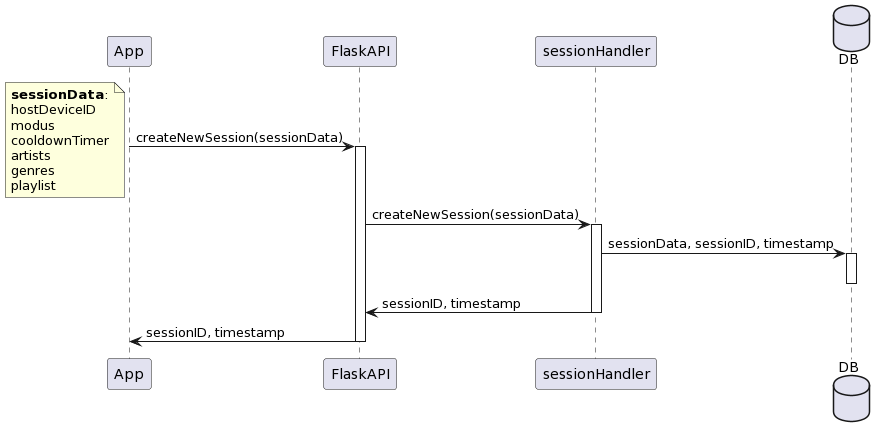
\includegraphics[width = 15cm]{LATEX/Entwurf/Graphics/createNewSession.png} 
\end{center}




\subsection*{deleteSession}

This method deletes a session by calling the deleteSession method of the sessionHandler. The sessionID is obtained from the userHandler by calling the getSessionIDByHostDeviceID method.

\textbf{Parameters:}

\begin{itemize}
    \item \textbf{hostDeviceID} (str): The deviceID of the host.
\end{itemize}

\textbf{Returns:}

\begin{itemize}
    \item None
\end{itemize}

\textbf{Raises:}

\begin{itemize}
    \item \textbf{error} (Session does not exist, or user is not host of the session): If the given user is not host of a session.
    \item \textbf{error} (sql error): If there is an error executing the SQL commands.
\end{itemize}

\begin{center}
   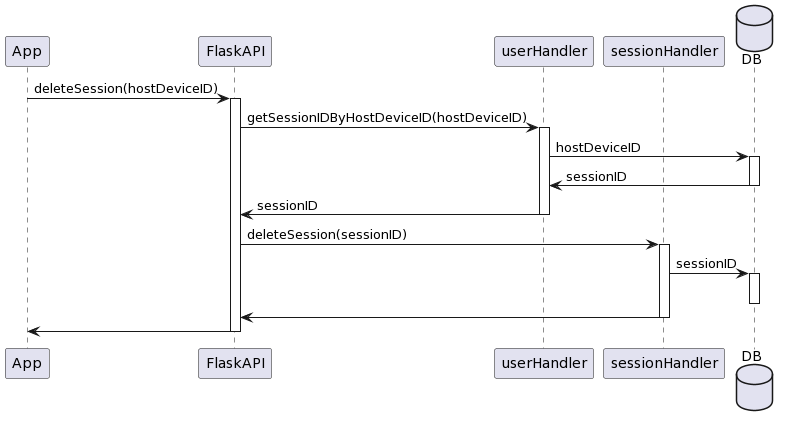
\includegraphics[width = 15cm]{LATEX/Entwurf/Graphics/deleteSession.png} 
\end{center}




\subsection*{getUserSessionState}

This method returns the user is an active participant, host or not a member of a session, by calling the getSessionIDByParticipantDeviceID and getSessionIDByHostDeviceID methods of the userHandler.

\textbf{Parameters:}

\begin{itemize}
    \item \textbf{deviceID} (str): The deviceID of the user.
\end{itemize}

\textbf{Returns:}

\begin{itemize}
    \item \textbf{userSessionState} (str (set(''NONE'', ''PARTICIPANT'', ''HOST''))): The userSessionState of the user.
\end{itemize}

\textbf{Raises:}

\begin{itemize}
    \item \textbf{error} (sql error): If there is an error executing the SQL commands.
\end{itemize}

\begin{center}
   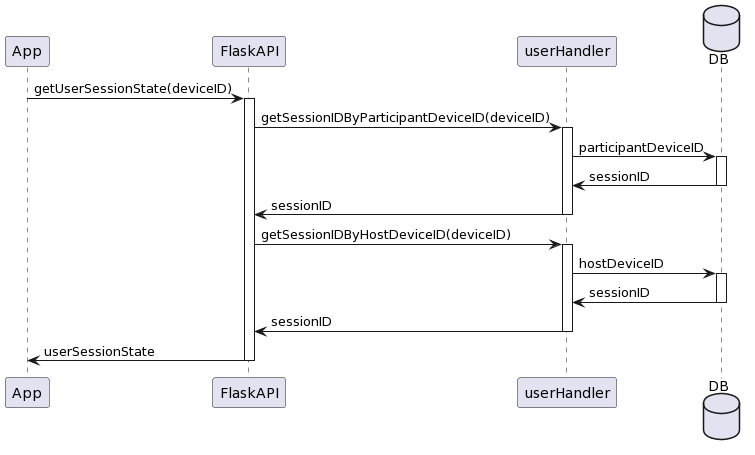
\includegraphics[width = 15cm]{LATEX/Entwurf/Graphics/getUserSessionState.png} 
\end{center}




\subsection*{getAllTrackData}

This method returns all tracks of the session, by calling the getTracksBySessionID method of the trackHandler.

\textbf{Parameters:}

\begin{itemize}
    \item \textbf{deviceID} (str): The deviceID of the user.
\end{itemize}

\textbf{Returns:}

\begin{itemize}
    \item \textbf{tracks} (array[track]): All tracks of the session.
\end{itemize}

\textbf{Raises:}

\begin{itemize}
    \item \textbf{error} (sql error): If there is an error executing the SQL commands.
\end{itemize}

\begin{center}
   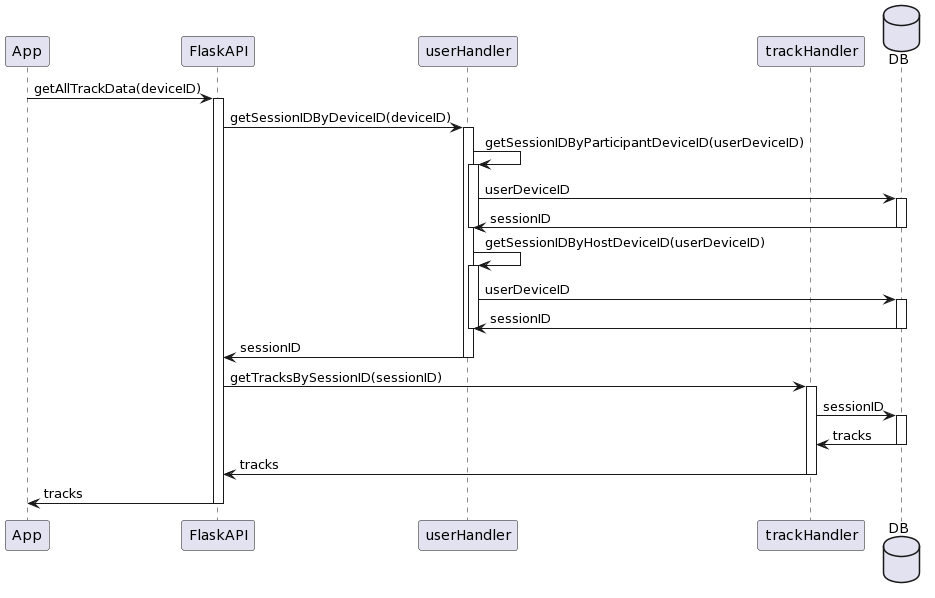
\includegraphics[width = 15cm]{LATEX/Entwurf/Graphics/getAllTrackData.png} 
\end{center}



\subsection*{getStatistics}

This method returns the most upvoted song, genre and artist, the total played tracks, the session duration, the total participants and the total upvotes of the session, by calling the getSessionStatsBySessionID method of the sessionHandler.

\textbf{Parameters:}

\begin{itemize}
    \item \textbf{deviceID} (str): The deviceID of the user.
\end{itemize}

\textbf{Returns:}

\begin{itemize}
    \item \textbf{mostUpvotedSong} (str): The most upvoted song of the session.
    \item \textbf{mostUpvotedGenre} (str): The most upvoted genre of the session.
    \item \textbf{mostUpvotedArtist} (str): The most upvoted artist of the session.
    \item \textbf{totalPlayedTracks} (int): The total played tracks of the session.
    \item \textbf{sessionDuration} (str): The duration of the session.
    \item \textbf{totalParticipants} (int): The total participants of the session.
    \item \textbf{totalUpvotes} (int): The total amount of upvotes of the session.
\end{itemize}

\textbf{Raises:}

\begin{itemize}
    \item \textbf{error} (sql error): If there is an error executing the SQL commands.
\end{itemize}

\begin{center}
   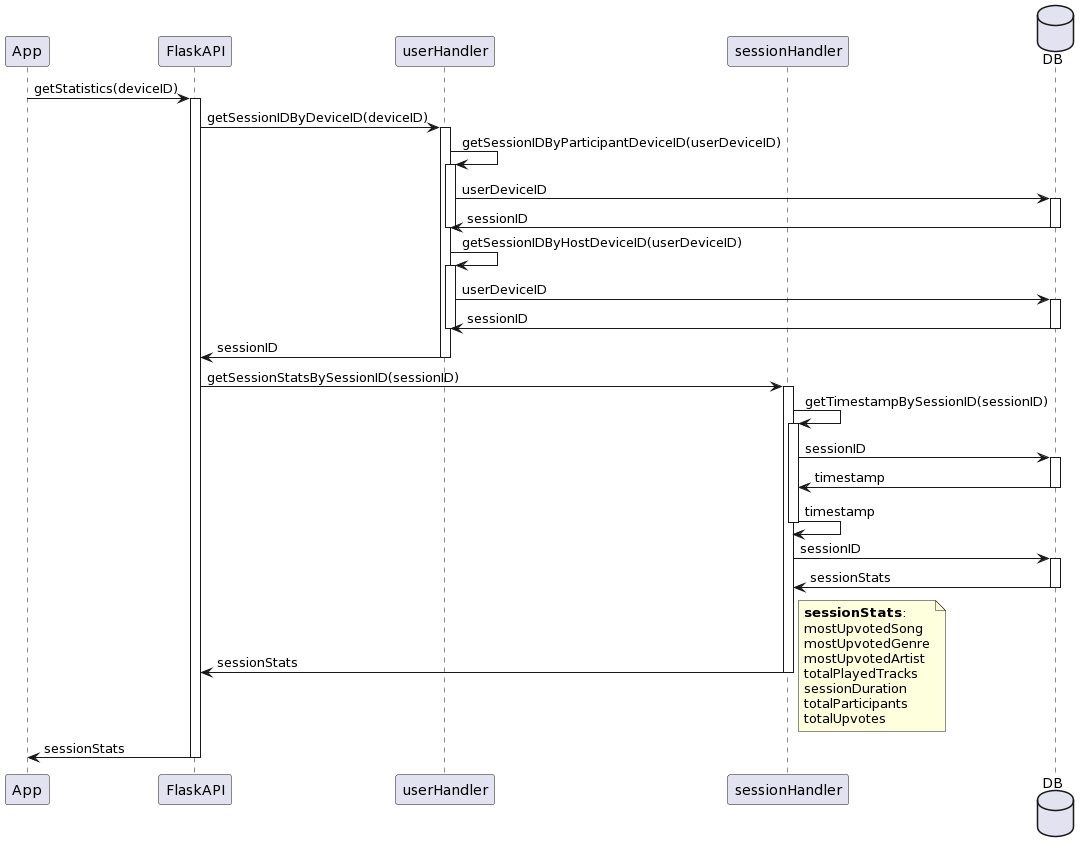
\includegraphics[width = 15cm]{LATEX/Entwurf/Graphics/getStatistics.png} 
\end{center}



\subsection*{participantJoinSession}

The method adds a participant to a session by calling the participantJoinSession method of the userHandler. The timestamp, modus, artists and genres of the session are obtained by calling the getSessionInfoBySessionID method of the sessionHandler.

\textbf{Parameters:}

\begin{itemize}
    \item \textbf{participantDeviceID} (str): The deviceID of the participant.
    \item \textbf{sessionID} (int (min 0, max 999999)): The ID of the session.
\end{itemize}

\textbf{Returns:}

\begin{itemize}
    \item \textbf{timestamp} (int): timestamp the session was created at, for unique identification.
    \item \textbf{modus} (str (set(''General'', ''Artist'', ''Genre'', ''Playlist''))): The modus of the session.
    \item \textbf{artists} (array[str]): All allowed artists of the session, only used in artistmode, otherwise null.
    \item \textbf{genres} (array[str]): All allowed genres of the session, only used in genremode, otherwise null.
\end{itemize}

\textbf{Raises:}

\begin{itemize}
    \item \textbf{error} (Participant is already in a session): If the given participant is already in a session.
    \item \textbf{error} (Session does not exist): If the given session does not exist.
    \item \textbf{error} (sql error): If there is an error executing the SQL commands.
\end{itemize}

\begin{center}
   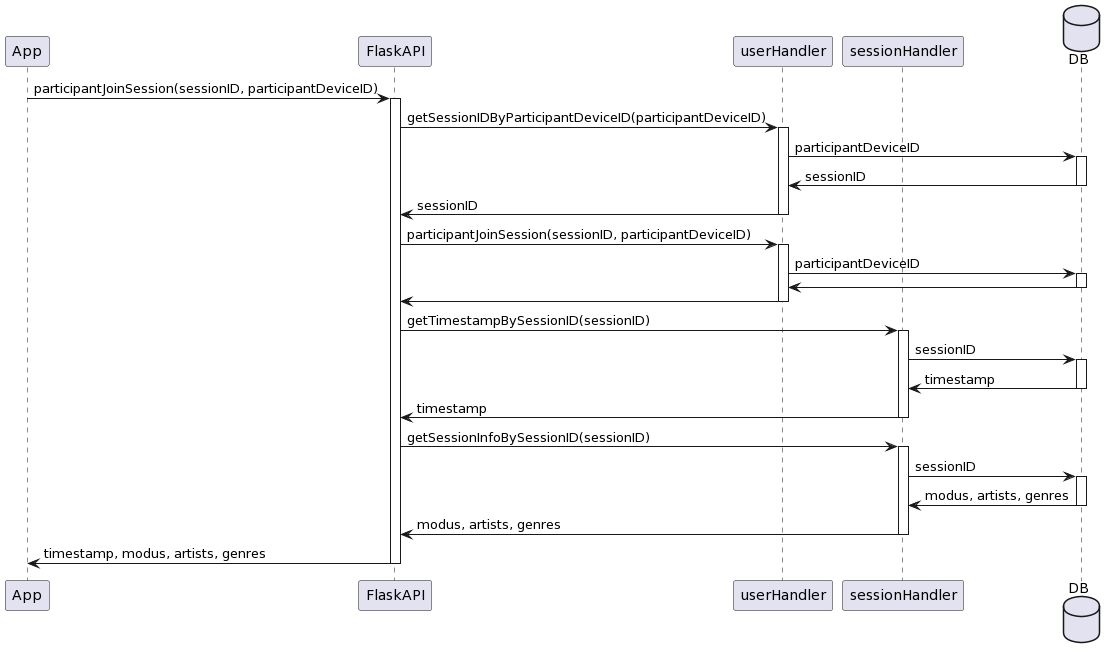
\includegraphics[width = 15cm]{LATEX/Entwurf/Graphics/participantJoinSession.png} 
\end{center}



\subsection*{participantLeaveSession}

The method sets a participant to inactive by calling the participantLeaveSession method of the userHandler.

\textbf{Parameters:}

\begin{itemize}
    \item \textbf{participantDeviceID} (str): The deviceID of the participant.
\end{itemize}

\textbf{Returns:}

\begin{itemize}
    \item None
\end{itemize}

\textbf{Raises:}

\begin{itemize}
    \item \textbf{error} (Participant is not in a session): If the given participant is not in a session.
    \item \textbf{error} (sql error): If there is an error executing the SQL commands.
\end{itemize}

\begin{center}
   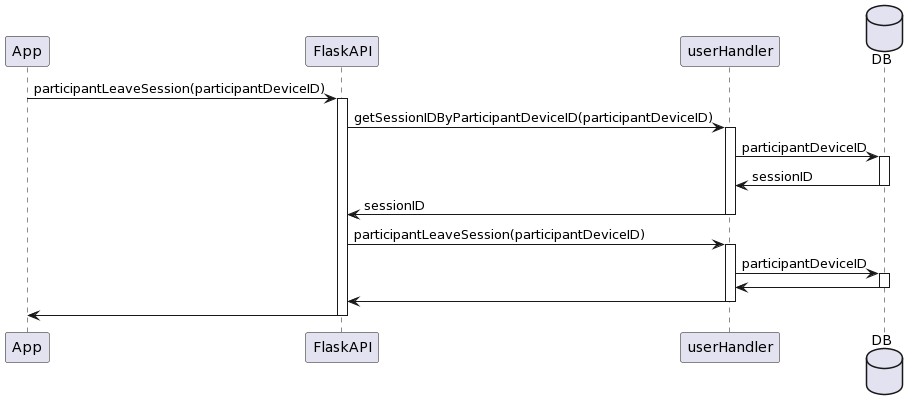
\includegraphics[width = 15cm]{LATEX/Entwurf/Graphics/participantLeaveSession.png} 
\end{center}



\subsection*{isSessionOpen}

The method checks if the session is still open by comparing the timestamp of the session with the timestamp of the request.

\textbf{Parameters:}

\begin{itemize}
    \item \textbf{sessionID} (int (min 0, max 999999)): The ID of the session.
    \item \textbf{timestamp} (int): timestamp the session was created at, for unique identification.
\end{itemize}

\textbf{Returns:}

\begin{itemize}
    \item \textbf{isOpen} (boolean): True if the session is still open, False otherwise.
\end{itemize}

\textbf{Raises:}

\begin{itemize}
    \item \textbf{error} (sql error): If there is an error executing the SQL commands.
\end{itemize}

\begin{center}
   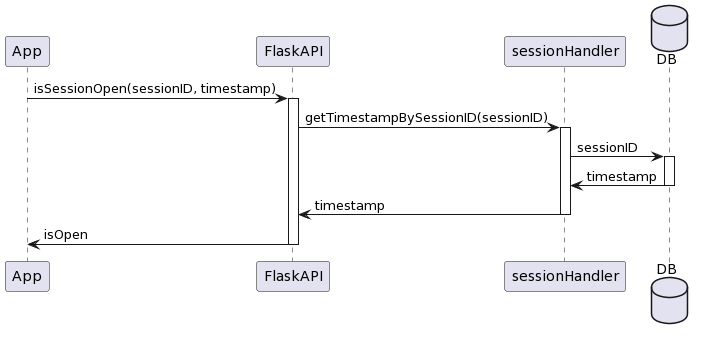
\includegraphics[width = 15cm]{LATEX/Entwurf/Graphics/isSessionOpen.png} 
\end{center}



\subsection*{addTrackToSession}

The method adds a track to the session by calling the addTrackToSession method of the trackHandler.

\textbf{Parameters:}

\begin{itemize}
    \item \textbf{deviceID} (str): The deviceID of the user.
    \item \textbf{trackID} (str): The ID of the track.
    \item \textbf{trackName} (str): The name of the track.
    \item \textbf{artist} (array[str]): The artists of the track.
    \item \textbf{genre} (array[str]): The genres of the track.
    \item \textbf{imageURL} (str): The image URL of the track.
\end{itemize}

\textbf{Returns:}

\begin{itemize}
    \item None
\end{itemize}

\textbf{Raises:}

\begin{itemize}
    \item \textbf{error} (sql error): If there is an error executing the SQL commands.
\end{itemize}


\begin{center}
   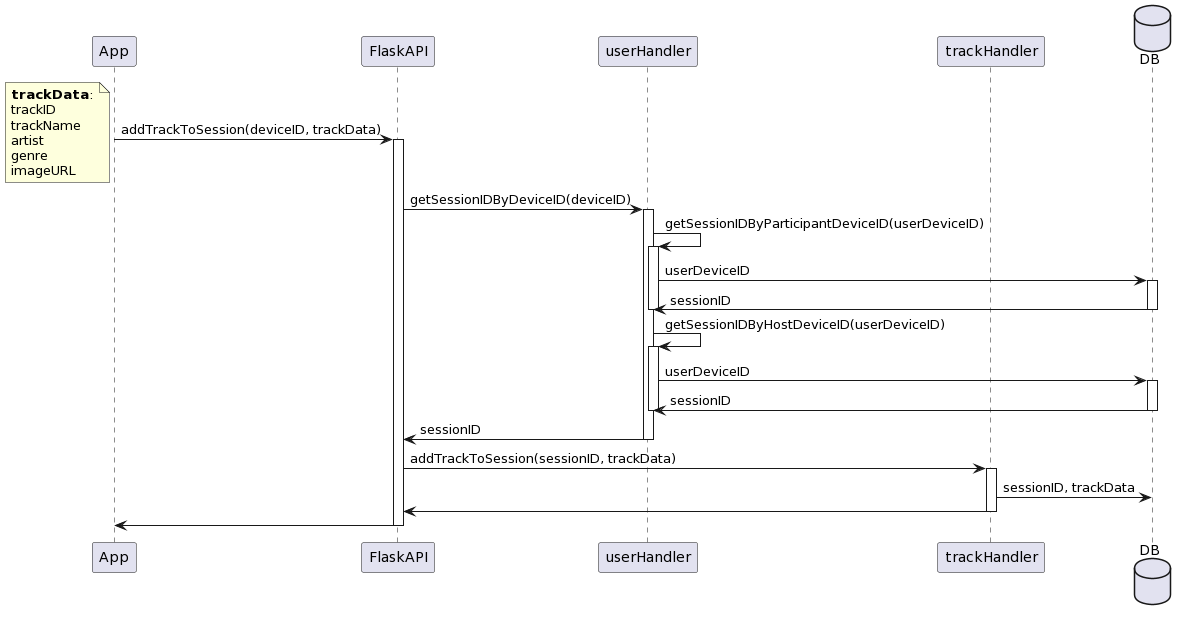
\includegraphics[width = 15cm]{LATEX/Entwurf/Graphics/addTrackToSession.png} 
\end{center}



\subsection*{addUpvoteToTrack}

The method adds an upvote to a track by calling the addVotesToTrack method of the trackHandler.

\textbf{Parameters:}

\begin{itemize}
    \item \textbf{deviceID} (str): The deviceID of the user.
    \item \textbf{trackID} (str): The ID of the track.
\end{itemize}

\textbf{Returns:}

\begin{itemize}
    \item None
\end{itemize}

\textbf{Raises:}

\begin{itemize}
    \item \textbf{error} (sql error): If there is an error executing the SQL commands.
\end{itemize}

\begin{center}
   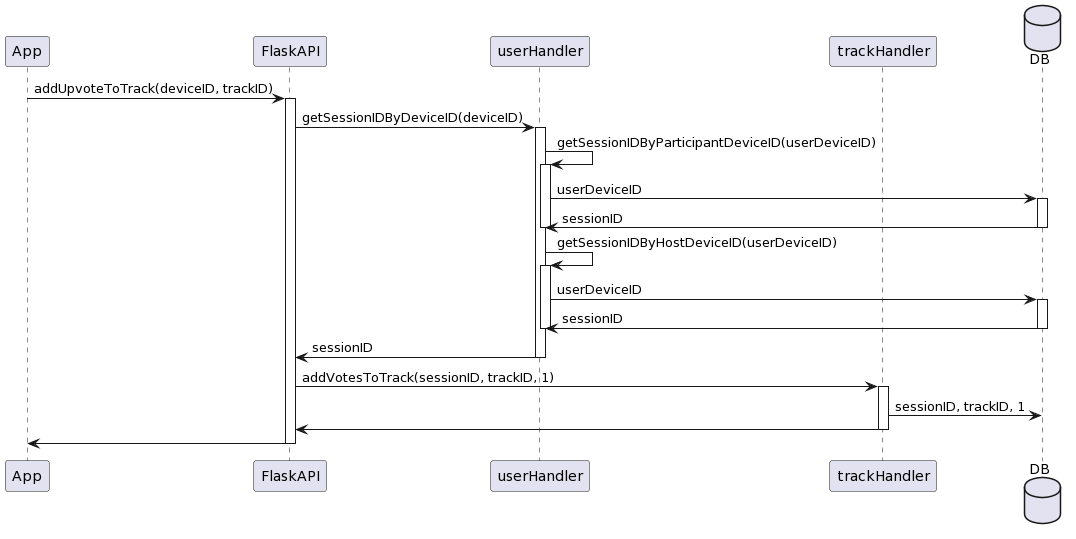
\includegraphics[width = 15cm]{LATEX/Entwurf/Graphics/addUpvoteToTrack.png} 
\end{center}



\subsection*{removeUpvoteFromTrack}

The method removes an upvote from a track by calling the addVotesToTrack method of the trackHandler.

\textbf{Parameters:}

\begin{itemize}
    \item \textbf{deviceID} (str): The deviceID of the user.
    \item \textbf{trackID} (str): The ID of the track.
\end{itemize}

\textbf{Returns:}

\begin{itemize}
    \item None
\end{itemize}

\textbf{Raises:}

\begin{itemize}
    \item \textbf{error} (sql error): If there is an error executing the SQL commands.
\end{itemize}

\begin{center}
   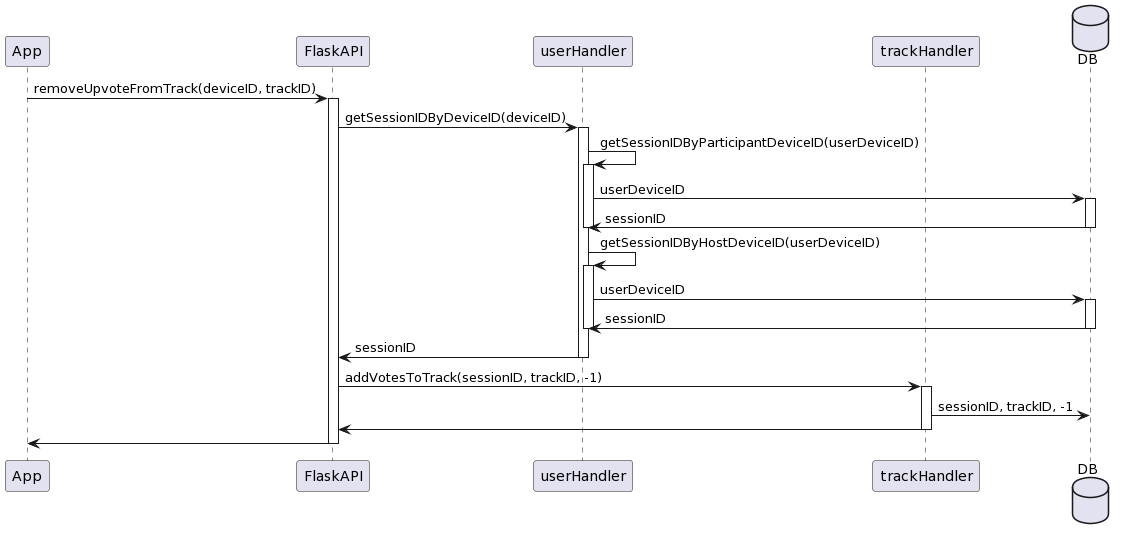
\includegraphics[width = 15cm]{LATEX/Entwurf/Graphics/removeUpvoteFromTrack.png} 
\end{center}



\subsection*{playedTrack}

The method resets the upvotes of a track, increments the total played tracks of the session and sets the cooldown start of the track to the current time, by calling the playedTrack method of the trackHandler.

\textbf{Parameters:}

\begin{itemize}
    \item \textbf{hostDeviceID} (str): The deviceID of the host.
    \item \textbf{trackID} (str): The ID of the track.
\end{itemize}

\textbf{Returns:}

\begin{itemize}
    \item None
\end{itemize}

\textbf{Raises:}

\begin{itemize}
    \item \textbf{error} (sql error): If there is an error executing the SQL commands.
\end{itemize}

\begin{center}
   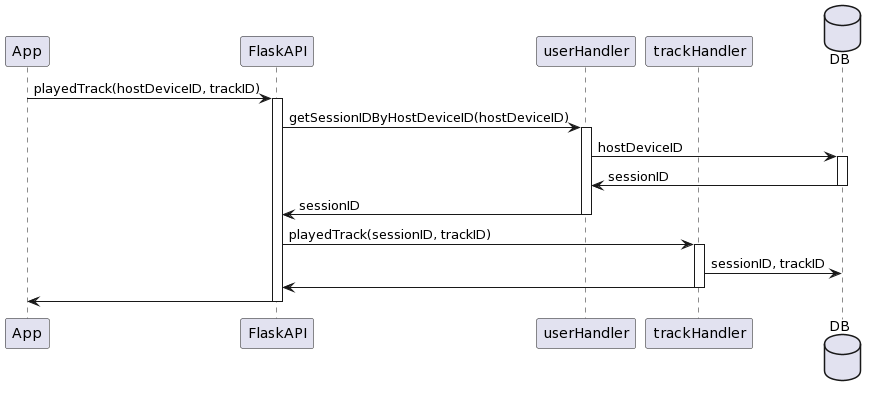
\includegraphics[width = 15cm]{LATEX/Entwurf/Graphics/playedTrack.png} 
\end{center}



\subsection*{setBlockTrack}

The method sets the blocked status of a track, by calling the setBlockTrack method of the trackHandler.

\textbf{Parameters:}

\begin{itemize}
    \item \textbf{hostDeviceID} (str): The deviceID of the host.
    \item \textbf{trackID} (str): The ID of the track.
    \item \textbf{blocked} (boolean): The blocked status of the track.
\end{itemize}

\textbf{Returns:}

\begin{itemize}
    \item None
\end{itemize}

\textbf{Raises:}

\begin{itemize}
    \item \textbf{error} (sql error): If there is an error executing the SQL commands.
\end{itemize}

\begin{center}
   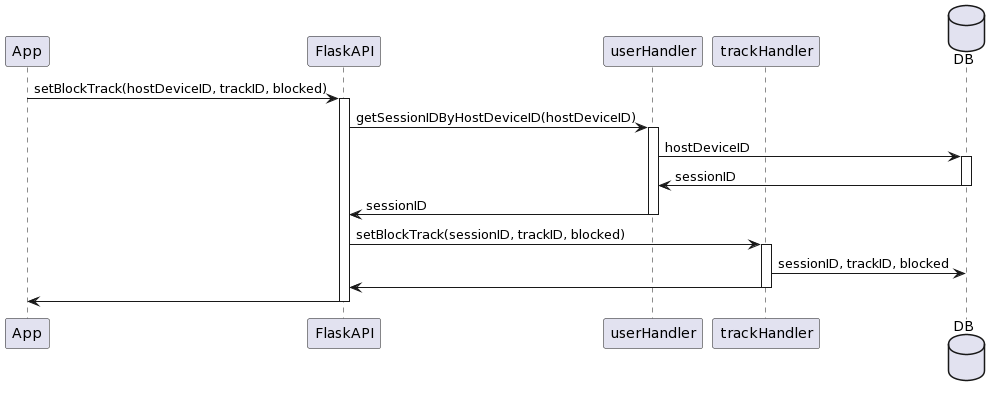
\includegraphics[width = 15cm]{LATEX/Entwurf/Graphics/setBlockTrack.png} 
\end{center}


\section{Database SQL Requests}

Die Methoden, welche SQL Requests an die Datenbank schicken, sind in die Klassen SessionHandler, UserHandler und TrackHandler aufgeteilt.

Die Funktionaliät um eine Verbindung zur Datenbank über Port 3306 herzustellen wird von dem Python Paket mariadb bereitgestellt. Die verwendete mariadb Version ist 1.1.9.

\subsection{sessionHandler}

\subsubsection{createNewSession}

This function creates a new session and returns the sessionID and the timestamp of the session. First a random sessionID is generated until an unused one is found. Then all session data is written to the database.

\textbf{Parameters}

\begin{itemize} \item \textbf{hostDeviceID} (int): The deviceID of the host. \item \textbf{modus} (int): The modus of the session. \item \textbf{cooldownTimer} (int): The cooldown timer of the session. \item \textbf{artists} (list): The artists of the session. \item \textbf{genres} (list): The genres of the session. \item \textbf{playlist} (list): The playlist of the session. \end{itemize}

\textbf{Returns}

\begin{itemize} \item \textbf{sessionID} (int): The ID of the session. \item \textbf{timestamp} (int): timestamp the session was created at. \end{itemize}

\textbf{Raises}

\begin{itemize} \item \textbf{mariadb.Error}: If there is an error executing the SQL commands. \end{itemize}

\subsubsection{deleteSession}

This function deletes the session with the given sessionID. First the session is deleted from the database. Then all participants are removed from the session. Then all tracks are removed from the session. If a track is not in any session anymore, it is removed from the global genre and artist list.

\textbf{Parameters}

\begin{itemize} \item \textbf{sessionID} (int): The ID of the session. \end{itemize}

\textbf{Returns}

\begin{itemize} \item None \end{itemize}

\textbf{Raises}

\begin{itemize} \item \textbf{mariadb.Error}: If there is an error executing the SQL commands. \end{itemize}

\subsubsection{getTimestampBySessionID}

This function returns the timestamp of the session with the given sessionID.

\textbf{Parameters}

\begin{itemize} \item \textbf{sessionID} (int): The ID of the session. \end{itemize}

\textbf{Returns}

\begin{itemize} \item \textbf{timestamp} (int): The timestamp of the session, or -1 if the session does not exist. \end{itemize}

\textbf{Raises}

\begin{itemize} \item \textbf{mariadb.Error}: If there is an error executing the SQL commands. \end{itemize}

\subsubsection{getSessionInfoBySessionID}

This function returns the modus, artists and genres of the session with the given sessionID. The artists and genres are returned as lists.

\textbf{Parameters}

\begin{itemize} \item \textbf{sessionID} (int): The ID of the session. \end{itemize}

\textbf{Returns}

\begin{itemize} \item \textbf{modus} (int): The modus of the session. \item \textbf{artists} (list): The allowed artists of the session. \item \textbf{genres} (list): The allowed genres of the session. \end{itemize}

\textbf{Raises}

\begin{itemize} \item \textbf{mariadb.Error}: If there is an error executing the SQL commands. \end{itemize}


\subsubsection{getSessionStatsBySessionID}

This function returns the most upvoted song, genre and artist, the total played tracks, the session duration, the total participants and the total upvotes of the session with the given sessionID.

\textbf{Parameters}

\begin{itemize}
    \item \textbf{sessionID} (int): The ID of the session.
\end{itemize}

\textbf{Returns}

\begin{itemize}
    \item \textbf{mostUpvotedSong} (string): The ID of the most upvoted song of the session.
    \item \textbf{mostUpvotedGenre} (string): The most upvoted genre of the session.
    \item \textbf{mostUpvotedArtist} (string): The most upvoted artist of the session.
    \item \textbf{totalPlayedTracks} (int): The total amount of played tracks of the session.
    \item \textbf{sessionDuration} (int): The duration of the session in minutes.
    \item \textbf{totalParticipants} (int): The total amount of participants of the session.
    \item \textbf{totalUpvotes} (int): The total amount of upvotes of the session.
\end{itemize}

\textbf{Raises}

\begin{itemize}
    \item \textbf{mariadb.Error}: If there is an error executing the SQL commands.
\end{itemize}



\subsection{userHandler}

\subsubsection{participantJoinSession}

This function adds the participant to the session if he is not already in it. If the participant was before in the session, he is set to active.

\textbf{Parameters}

\begin{itemize}
    \item \textbf{participantDeviceID} (int): The ID of the participant.
    \item \textbf{sessionID} (int): The ID of the session.
\end{itemize}

\textbf{Returns}

\begin{itemize}
    \item None
\end{itemize}

\textbf{Raises}

\begin{itemize}
    \item \textbf{mariadb.Error}: If there is an error executing the SQL commands.
\end{itemize}

\subsubsection{participantLeaveSession}

This function removes the participant from the session that he is currently in. If the participant is not in a session, nothing happens.

\textbf{Parameters}

\begin{itemize}
    \item \textbf{participantDeviceID} (int): The ID of the participant.
\end{itemize}

\textbf{Returns}

\begin{itemize}
    \item None
\end{itemize}

\textbf{Raises}

\begin{itemize}
    \item \textbf{mariadb.Error}: If there is an error executing the SQL commands.
\end{itemize}

\subsubsection{getSessionIDByParticipantDeviceID}

This function returns the sessionID if the given user is active participant of a session, -1 otherwise.

\textbf{Parameters}

\begin{itemize}
    \item \textbf{participantDeviceID} (int): The ID of the participant.
\end{itemize}

\textbf{Returns}

\begin{itemize}
    \item \textbf{sessionId} (int): The ID of the session, -1 if the participant is not in an active session.
\end{itemize}

\textbf{Raises}

\begin{itemize}
    \item \textbf{mariadb.Error}: If there is an error executing the SQL commands.
\end{itemize}

\subsubsection{getSessionIDByHostDeviceID}

This function returns the sessionID if the given user is host of a session, -1 otherwise.

\textbf{Parameters}

\begin{itemize}
    \item \textbf{hostDeviceID} (int): The ID of the host.
\end{itemize}

\textbf{Returns}

\begin{itemize}
    \item \textbf{sessionId} (int): The ID of the session, -1 if the host is not in a session.
\end{itemize}

\textbf{Raises}

\begin{itemize}
    \item \textbf{mariadb.Error}: If there is an error executing the SQL commands.
\end{itemize}

\subsubsection{getSessionIDByDeviceID}

This function returns the sessionID if the given user is host or active participant of a session, -1 otherwise.

\textbf{Parameters}

\begin{itemize}
    \item \textbf{userDeviceID} (int): The ID of the user.
\end{itemize}

\textbf{Returns}

\begin{itemize}
    \item \textbf{sessionId} (int): The ID of the session, -1 if the user is not in a session.
\end{itemize}



\subsection{trackHandler}

\subsubsection{getTracksBySessionID}

This function returns the trackID, trackName, upvotes, artists, imageURL, isBlocked and onCooldown of all tracks in the session. The artists are returned as a list.

\textbf{Parameters}

\begin{itemize} \item \textbf{sessionID} (int): The ID of the session. \end{itemize}

\textbf{Returns}

\begin{itemize} \item \textbf{tracklist} (list(tracks)): The list of tracks in the session. \end{itemize}

\textbf{Raises}

\begin{itemize} \item \textbf{mariadb.Error}: If there is an error executing the SQL commands. \end{itemize}

\subsubsection{addTrackToSession}

This function adds a track to the session, if it is not already in the session. The artists and genres are added to the global artist and genre list, if they are not already in the list.

\textbf{Parameters}

\begin{itemize} \item \textbf{sessionID} (int): The ID of the session. \item \textbf{trackID} (int): The ID of the track. \item \textbf{trackName} (string): The name of the track. \item \textbf{artists} (list(string)): The list of artists of the track. \item \textbf{genres} (list(string)): The list of genres of the track. \item \textbf{imageURL} (string): The URL of the image of the track. \end{itemize}

\textbf{Returns}

\begin{itemize} \item None \end{itemize}

\textbf{Raises}

\begin{itemize} \item \textbf{mariadb.Error}: If there is an error executing the SQL commands. \end{itemize}

\subsubsection{addVotesToTrack}

This function adds the given amount of upvotes to a track. If the amount of upvotes is negative, the upvotes are subtracted.

\textbf{Parameters}

\begin{itemize} \item \textbf{sessionID} (int): The ID of the session. \item \textbf{trackID} (int): The ID of the track. \item \textbf{amount} (int): The amount of upvotes to add. \end{itemize}

\textbf{Returns}

\begin{itemize} \item None \end{itemize}

\textbf{Raises}

\begin{itemize} \item \textbf{mariadb.Error}: If there is an error executing the SQL commands. \end{itemize}

\subsubsection{playedTrack}

This function sets the upvotes of the track to the given trackID to 0, sets the cooldown start of the track to the current time and increments the amount played of the track by one.

\textbf{Parameters}

\begin{itemize} \item \textbf{sessionID} (int): The ID of the session. \item \textbf{trackID} (int): The ID of the track. \end{itemize}

\textbf{Returns}

\begin{itemize} \item None \end{itemize}

\textbf{Raises}

\begin{itemize} \item \textbf{mariadb.Error}: If there is an error executing the SQL commands. \end{itemize}

\subsubsection{setBlockTrack}

This function sets the blocked status of the track to the given trackID to the given status.

\textbf{Parameters}

\begin{itemize} \item \textbf{sessionID} (int): The ID of the session. \item \textbf{trackID} (int): The ID of the track. \item \textbf{blocked} (boolean): The blocked status of the track. \end{itemize}

\textbf{Returns}

\begin{itemize} \item None \end{itemize}

\textbf{Raises}

\begin{itemize} \item \textbf{mariadb.Error}: If there is an error executing the SQL commands. \end{itemize}





\chapter{Datenbank}
\label{chap:Datenbank}

\begin{figure}[h]
    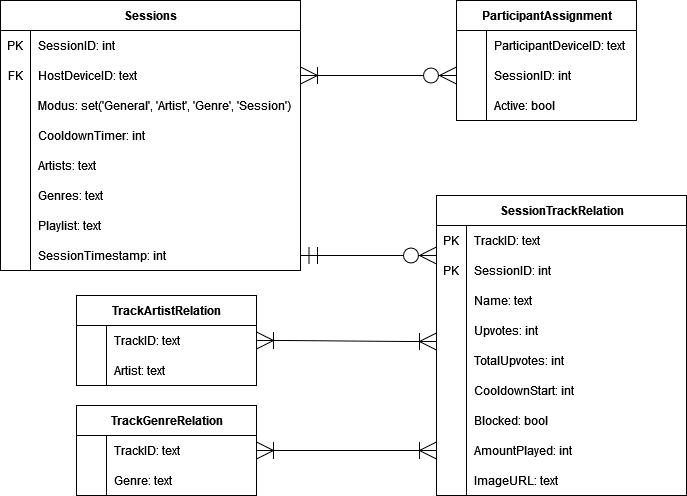
\includegraphics[width = 16cm]{LATEX/Entwurf/Graphics/ER-Diagram.png}
    \caption{ER-Diagramm}
    \label{fig:ER-Diagramm}
\end{figure}

\section{ParticipantAssignment}

Stores the relevant data for a participant of a section.

\begin{itemize}
    \item \textbf{ParticipantDeviceID} (text): The specific ID of the participant.
    \item \textbf{SessionID} (int): The specific ID of the session the participant is in.
    \item \textbf{Active} (bool): States if the participant is active in this session.
\end{itemize}

\section{Sessions}

Stores the relevant data of a session.

\begin{itemize}
    \item \textbf{SessionID} (int): The specific ID of the session.
    \item \textbf{HostDeviceID} (text): The specific ID of the host of this session.
    \item \textbf{Modus} (set): The mode of the session.
    \item \textbf{CooldownTimer} (int): The cooldown timer for played tracks.
    \item \textbf{Artists} (text): The allowed artists in the artist mode.
    \item \textbf{Genres} (text): The allowed genres in the genre mode.
    \item \textbf{Playlist} (text): The deposited playlist for the session.
    \item \textbf{SessionTimestamp} (int): The timestamp indicating the time the session was created at.
\end{itemize}

\section{SessionTrackRelation}

Stores the data that is important for the relation between a session and its tracks.

\begin{itemize}
    \item \textbf{TrackID} (text): The specific ID of the track in the relation.
    \item \textbf{SessionID} (int): The specific ID of the session in the relation.
    \item \textbf{Name} (text): The name of the track.
    \item \textbf{Upvotes} (int): The amount of upvotes of the track while it is in the suggestion list and not played.
    \item \textbf{TotalUpvotes} (int): The total amount of upvotes of the track during the entire session.
    \item \textbf{CooldownStart} (int): The time the track is played and its cooldown starts.
    \item \textbf{Blocked} (bool): States if the track is blocked and cannot be upvoted.
    \item \textbf{AmountPlayed} (int): The total count of how often the track was played in the entire session.
    \item \textbf{ImageURL} (text): The image of the track as URL.
\end{itemize}

\section{TrackArtistRelation}

Stores the data that is important for the relation between a track and its artists.

\begin{itemize}
    \item \textbf{TrackID} (text): The specific ID of the track in the relation.
    \item \textbf{Artist} (text): The artist in the relation.
\end{itemize}

\section{TrackGenreRelation}

Stores the data that is important for the relation between a track and its genres.

\begin{itemize}
    \item \textbf{TrackID} (text): The specific ID of the track in the relation.
    \item \textbf{Genre} (text): The genre in the relation.
\end{itemize}

\chapter{Sequenzdiagramme}
\label{chap:Sequenzdiagramme}

In den nachfolgenden Sequenzdiagrammen werden ausgewählte Abläufe innerhalb des gesamten Systems gesondert dargestellt.
\vspace{1cm}

\begin{figure}[h]
    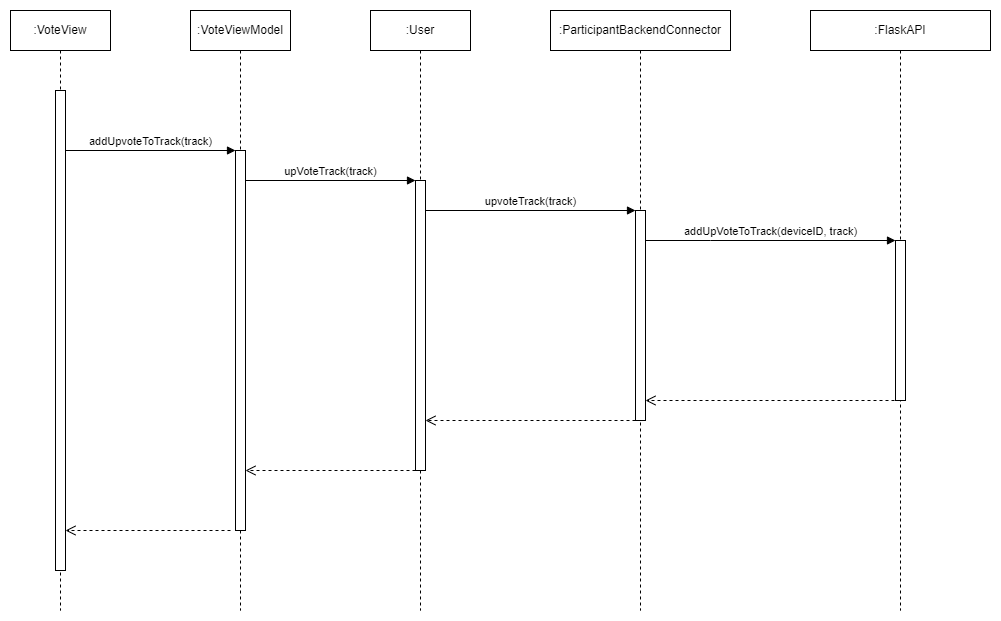
\includegraphics[width = 16cm]
{LATEX/Entwurf/Graphics/sequenzdiagramm_01.png}
    \caption{Track upvoten}
    \label{fig:sequenzdiagramm01}
\end{figure}

\vspace{1cm}
Ausgangspunkt ist hier die VoteView. Wird auf dieser per dazugehörigem Button ein Upvote für einen Track ausgelöst, so wird dieser Befehl über den entsprechenden User und den dazugehörigen ParticipantConnector an das Backend weitergereicht und dort registriert. 



\begin{figure}[h]
    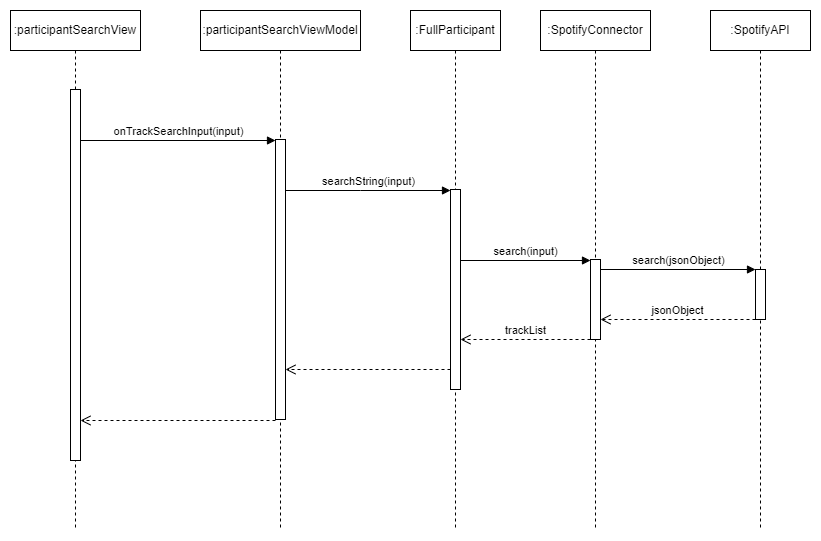
\includegraphics[width = 16cm]
{LATEX/Entwurf/Graphics/sequenzdiagramm_02.png}
    \caption{Tracksuche mit der Spotify-API}
    \label{fig:sequenzdiagramm02}
\end{figure}

\vspace{6cm}
Abb. 6.2 veranschaulicht den Ablauf der Suche nach Tracks im Zusammenspiel mit der Spotify-API, Ausgangspunkt ist die participantSearchView. Der gewählte Session-Modus ist hier der General Mode. Während des Ablaufs werden Eingaben im Suchfeld erkannt, woraufhin die Eingabedaten weitergereicht und an die Spotify-API gesendet werden, welche im Anschluss mittels einer API-Abfrage das gewünschte Suchergebnis liefert.




\end{document}


